\documentclass[journal]{IEEEtran}
\usepackage[T1]{fontenc}
\usepackage[utf8]{inputenc}
\usepackage{amsmath,amssymb,mathtools}
\usepackage{graphicx}
\usepackage{booktabs,array,multirow}
\usepackage{xcolor}
\usepackage{cite}
\usepackage{url}
\usepackage{tikz}
\usetikzlibrary{arrows.meta,positioning,shapes.geometric,fit}
\graphicspath{{figures/}}
\newcommand{\todo}[1]{\textcolor{red}{[TODO: #1]}}
\newcommand{\mua}{\mu_a}
\newcommand{\mus}{\mu_s}
\newcommand{\musp}{\mu_s'}
\newcommand{\mut}{\mu_t}
\newcommand{\lex}{\lambda_{\mathrm{ex}}}
\newcommand{\lem}{\lambda_{\mathrm{em}}}
\DeclareMathOperator{\diag}{diag}
\DeclareMathOperator{\tr}{tr}
\hyphenation{Spectral-Forge}

\begin{document}
\title{SpectralForge Studio: A Physically Comprehensive Multi-Excitation Fluorescence Hyperspectral Simulator and Experiment-Design Toolkit for Layered Tissue}
\author{Narek~Meloyan and Narine~Sarvazyan%
\thanks{N. Meloyan is with the Akian College of Science and Engineering and the Engineering Research Center, American University of Armenia, Yerevan, Armenia, and the L.A.\ Orbeli Institute of Physiology NAS RA, Yerevan, Armenia (e-mail: narek.h.meloyan@gmail.com).}%
\thanks{N. Sarvazyan is with the Akian College of Science and Engineering, American University of Armenia, the L.A.\ Orbeli Institute of Physiology NAS RA, Yerevan, Armenia, and George Washington University, Washington, DC, USA (e-mail: phynas@gwu.edu).}}
\markboth{IEEE Transactions on Computational Imaging, manuscript draft}{Meloyan and Sarvazyan: SpectralForge Studio}
\maketitle

\begin{abstract}
Multi-excitation fluorescence hyperspectral imaging (ME-HSI) records an excitation--emission matrix at every pixel, but the signal of a buried fluorophore is distorted by the tissue above it, and real acquisitions carry no ground truth. We present SpectralForge Studio, an open simulator and experiment-design environment for ME-HSI of layered tissue. It combines a 3D scene editor, a forward model (ray optics, dye photophysics, a layered-block 3D Monte Carlo with voxel inclusions, a tissue-optics library, a tunable-filter camera chain) and a research toolkit: sensitivity analysis, unmixing, maximum-likelihood retrieval, Fisher-information analysis with a model-error term and channel selection, and calibration of a digital twin. The transport engine reproduces the MCML benchmark to $0.1\,\%$, conserves energy to $10^{-9}$ and matches an independent Monte Carlo for radial reflectance to $1\,\%$. A calibrated twin predicts held-out excitation lines of measured collagen spectra with a mean spectral angle of $8.4^\circ$ (nominal instrument $14.2^\circ$), though not better than a copy of a measured spectrum ($7.7^\circ$). In simulations of collagen-covered tissue, the buried signal decays with an effective depth of $0.07$--$0.36$~mm for 340--430~nm excitation; cover parameters carry a first-order share of $0.66$ of the optical redox-ratio variance against $0.16$ for NADH and FAD; about 30 of 248 channels come within $10\,\%$ of the full-protocol Cram\'er--Rao bound, yet thickness retrieval is limited by model error (RMSE $160$--$260$~\textmu m), not photon noise; and unmixing with a thin-cover library fails from $0.1$~mm depth. The software is open source.
\end{abstract}

\begin{IEEEkeywords}
Fluorescence hyperspectral imaging, Monte Carlo light transport, tissue optics, simulation, experiment design, Fisher information, sensitivity analysis, digital twin.
\end{IEEEkeywords}

\section{Introduction}
\IEEEPARstart{M}{ulti-excitation} fluorescence hyperspectral imaging (ME-HSI) illuminates a sample at several excitation wavelengths and records, for each, an emission spectrum in many bands. Every pixel thus carries an excitation--emission matrix (EEM) and an image is a four-dimensional array over excitation, emission, height and width. The joint domain separates fluorophores that a single excitation cannot, which is why endogenous autofluorescence from NADH, FAD, collagen and elastin has been used for label-free imaging of tissue state~\cite{zipfel2003,georgakoudi2012,croce2014,ramanujam2000}, including cardiac ablation lesions~\cite{mercader2012,gil2017,guan2018} and tissue classification with ME-HSI~\cite{chil4d2025,chillichen2025,hunanyan2025}. A particularly important derived quantity is the optical redox ratio, built from the FAD and NADH signals, which tracks cellular metabolism~\cite{skala2007,georgakoudi2012}.

Tissue is rarely imaged bare. In many applications the fluorophore of interest sits under a cover that scatters, absorbs and fluoresces itself: a collagen-rich layer, an epithelium, a blood-perfused dermis. The cover attenuates the excitation on the way in and the emission on the way out, adds its own autofluorescence, and, because haemoglobin absorbs strongly in the violet and green, \emph{distorts the emission spectrum} rather than merely scaling it~\cite{wu1993,muller2001}. A ratio such as FAD/(FAD+NADH) is therefore not a pure property of the metabolic state. Quantifying how much of its variance is caused by the cover, and designing acquisitions and estimators that are robust to it, requires ground truth that real measurements cannot supply: the true thickness, concentrations and optical properties of every pixel.

Simulation is the natural remedy, and it serves three purposes. (i) It supplies \emph{ground truth} for developing and benchmarking processing methods. (ii) It supports \emph{experiment design}, i.e. choosing excitation lines, emission bands, exposure and geometry before instrument time is spent; each added excitation multiplies acquisition time and photobleaches the sample. (iii) It enables \emph{inverse problems}: parameter retrieval, unmixing and uncertainty quantification with a forward model that is faithful enough to be inverted.

\subsection{Gaps}
Photon-transport codes are mature~\cite{wang1995mcml,fang2009mcx,shen2010timos,leino2019valomc}, but they are solvers: they return fluence, reflectance or absorption for a given set of optical properties. A user who wants to simulate an \emph{imaging experiment} must still add the excitation source and its line shape, dye photophysics (inner filter, quenching, FRET, bleaching, Raman), the emission transport, the tunable-filter bands and the detector noise, and then wrap everything in a design-of-experiments and inference pipeline. Hyperspectral scene simulators for remote sensing~\cite{goodenough2017dirsig} cover the camera and scene but not fluorescence transport in turbid media. Our previous simulator~\cite{meloyan2026spectraforge} generated labelled 4D fluorescence cubes with a one-dimensional transport model; it could not represent a cover whose thickness varies laterally, light spreading sideways, or buried inclusions, and it offered no study or inference tools.

\subsection{Contributions}
\begin{enumerate}
\item \textbf{A schema-first, end-to-end ME-HSI simulator} with a 3D scene editor, a headless Python API and a command-line interface that share one typed experiment contract (Section~\ref{sec:system}).
\item \textbf{A physically comprehensive forward model}: ray optics with Fresnel/Snell and microfacet glint, dye photophysics, white-Monte-Carlo transport kernels with reciprocity, and a layered-block 3D Monte Carlo with layer-conforming tallies, a peel-off estimator with multiple-importance weights, voxelised inclusions, and a literature tissue-optics model (Section~\ref{sec:physics}).
\item \textbf{A research toolkit}: a study engine with provenance, Sobol'/Morris sensitivity, unmixing, surrogate maximum-likelihood retrieval, Fisher-information/CRLB analysis with D-optimal channel selection, and calibration of a digital twin (Section~\ref{sec:toolkit}).
\item \textbf{A validation suite} against analytic and published references, including a check of the voxel inclusions against an independent Monte Carlo, and a sim-to-real study with measured collagen and droplet data (Section~\ref{sec:validation}).
\item \textbf{A set of simulation experiments} on collagen-covered tissue that quantify attenuation and spectral distortion, confounding of the redox ratio, information-optimal acquisition and its limits under model error, thickness retrieval, depth-dependent unmixing failure and label-free segmentation (Section~\ref{sec:experiments}). \todo{add inclusion detectability (E4) and performance (E10) when complete}
\end{enumerate}

\section{Related Work}
\label{sec:related}
\textbf{Tissue-optics Monte Carlo.} MCML~\cite{wang1995mcml} established the standard for multilayered tissue with implicit capture, Henyey--Greenstein scattering~\cite{henyey1941} and Fresnel boundaries; the same ideas are reviewed in~\cite{jacques2011mc,jacques2008tutorial}, and voxelised variants such as mcxyz extend them to heterogeneous media. GPU implementations followed, for layered media~\cite{alerstam2008} and for voxel media~\cite{fang2009mcx}. Complex boundaries are handled by mesh-based codes~\cite{boas2002,fang2010mmc,shen2010timos,leino2019valomc} and hybrid mesh--voxel methods~\cite{yan2020hybrid}. Our engine is closest to MCML in its formulation (Section~\ref{sec:mc3d}) but is extended to tilted planar interfaces, voxel inclusions and an excitation/emission two-pass structure with a next-event estimator; it is not a general-purpose replacement for mesh-based codes.

\textbf{Fluorescence Monte Carlo.} Fluorescence propagation was modelled by Welch \emph{et al.}~\cite{welch1997} and Jacques~\cite{jacques2003fluor}; accelerated schemes for layered tissue~\cite{swartling2003} and time-resolved fluorescence~\cite{liebert2008} reduce the cost by reusing the excitation transport. We follow the same decomposition, but add quantitative dye photophysics and the full camera chain, and we resolve photobleaching per voxel across an excitation sequence.

\textbf{Hyperspectral scene simulators.} DIRSIG~\cite{goodenough2017dirsig} is the best-known physics-based image simulator for remote sensing, with a rich sensor model but without fluorescence in turbid media. Domain randomisation~\cite{tobin2017} uses synthetic data for sim-to-real transfer in robotics; we instead calibrate a physical model to measured data.

\textbf{Fluorescence EEM analysis and unmixing.} EEM data are classically analysed with multi-way models such as PARAFAC~\cite{bro1997,murphy2013}; in imaging, linear unmixing of spectral images is established~\cite{zimmermann2005,keshava2002,bioucas2012}, with constrained solvers~\cite{heinz2001,lawson1995} and endmember extraction by NMF~\cite{lee1999} or vertex component analysis~\cite{nascimento2005}. Tunable-filter spectral imaging is reviewed in~\cite{morris1994lctf,lu2014,valm2017}.

\textbf{Intrinsic fluorescence in turbid media.} Wu \emph{et al.}~\cite{wu1993} and M\"uller \emph{et al.}~\cite{muller2001} showed how scattering and absorption distort measured fluorescence relative to the intrinsic spectrum, and Richards-Kortum and Sevick-Muraca~\cite{richards1996} reviewed quantitative tissue spectroscopy. Our simulator reproduces such distortions from first principles, so that correction strategies can be tested against known ground truth.

\textbf{Global sensitivity analysis.} Variance-based Sobol' indices~\cite{sobol2001,saltelli2010,jansen1999} and Morris screening~\cite{morris1991,campolongo2007} are standard in computational modelling. We expose them as first-class operations on simulated imaging experiments and report the Monte Carlo noise floor of the indices.

\textbf{Experiment design and band selection.} Optimal experimental design maximises functionals of the Fisher information matrix~\cite{pukelsheim2006}; greedy maximisation of monotone submodular criteria has a $1-1/e$ guarantee~\cite{nemhauser1978}. In hyperspectral imaging, band selection is usually data-driven~\cite{chang1999,sun2019bandselection,cai2020bsnets,meloyan2025scirep}. Here the forward model is known, so channel selection can be posed as a model-based design problem and compared with data-driven selectors.

\textbf{Digital twins.} Digital twins couple a model with measurements of a specific physical asset~\cite{rasheed2020,katsoulakis2024}. We use the term in this restricted sense: a forward model whose instrument and fluorophore parameters are calibrated to laboratory data, with explicit statements of what is and is not identifiable.

\section{System}
\label{sec:system}
SpectralForge Studio consists of a typed experiment contract, a Python engine and a web application (Fig.~\ref{fig:arch}).

\begin{figure*}[!t]
\centering
\resizebox{0.95\textwidth}{!}{%
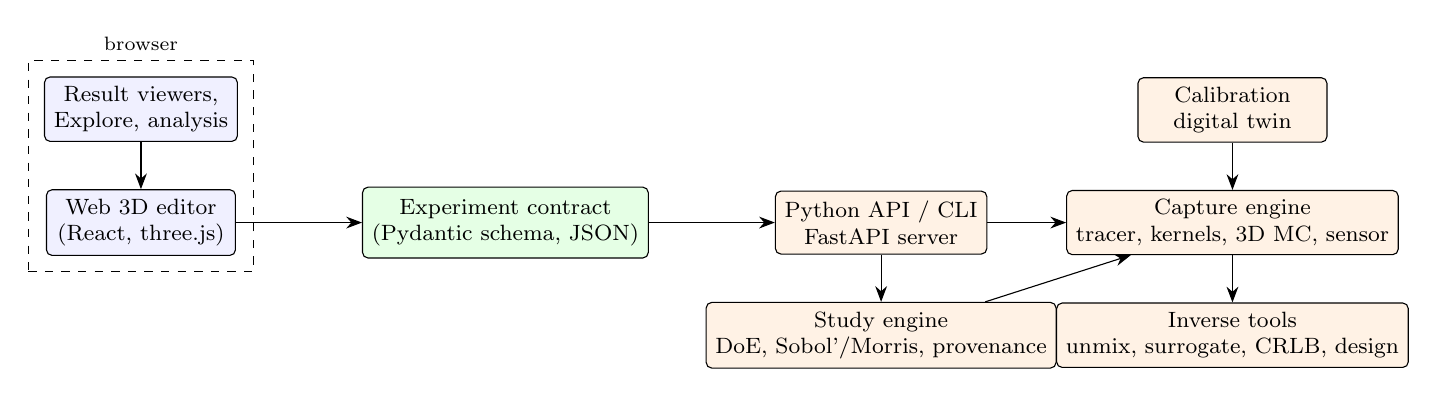
\begin{tikzpicture}[font=\footnotesize,node distance=6mm and 10mm,
 box/.style={draw,rounded corners=2pt,minimum height=8mm,minimum width=24mm,align=center,fill=blue!6},
 eng/.style={draw,rounded corners=2pt,minimum height=8mm,minimum width=24mm,align=center,fill=orange!10},
 ct/.style={draw,rounded corners=2pt,minimum height=9mm,minimum width=34mm,align=center,fill=green!10},
 arr/.style={-{Stealth[length=2mm]}}]
\node[ct] (schema) {Experiment contract\\(Pydantic schema, JSON)};
\node[box,left=of schema,xshift=-6mm] (web) {Web 3D editor\\(React, three.js)};
\node[box,above=of web] (mock) {Result viewers,\\Explore, analysis};
\node[eng,right=of schema,xshift=6mm] (api) {Python API / CLI\\FastAPI server};
\node[eng,right=of api] (cap) {Capture engine\\tracer, kernels, 3D MC, sensor};
\node[eng,below=of api] (study) {Study engine\\DoE, Sobol'/Morris, provenance};
\node[eng,below=of cap] (inv) {Inverse tools\\unmix, surrogate, CRLB, design};
\node[eng,above=of cap] (cal) {Calibration\\digital twin};
\draw[arr] (web) -- (schema); \draw[arr] (schema) -- (api); \draw[arr] (api) -- (cap);
\draw[arr] (api) -- (study); \draw[arr] (study) -- (cap); \draw[arr] (cap) -- (inv); \draw[arr] (cal) -- (cap);
\draw[arr] (mock) -- (web);
\node[draw,dashed,fit={(web)(mock)},inner sep=2mm,label={[font=\scriptsize]above:browser}] {};
\end{tikzpicture}}
\caption{Architecture of SpectralForge Studio. The experiment contract is defined once in Python and exported as JSON Schema and TypeScript types for the browser, so the editor and the engine cannot diverge. \todo{replace the sketch with the final architecture diagram}}
\label{fig:arch}
\end{figure*}

\textbf{Schema-first contract.} An experiment is a single Pydantic object holding fluorophores, materials (each a uniform optical medium), objects, a background, light sources with excitation sequences, cameras and acquisition settings including the physics toggles. The schema is exported to JSON Schema and TypeScript, so the browser editor builds only experiments that validate in the engine. The experiment is embedded verbatim in every exported cube, together with a provenance record (package and library versions, git commit and dirty flag, seed and the SHA-256 hash of the canonical experiment JSON), so any result can be traced to its configuration.

\textbf{Engine.} The engine is written in Python with numba-compiled kernels. A capture first traces camera rays through analytic solids into a wavelength-independent hit buffer, then assembles the spectral radiance for each excitation step from per-material optics and the transport kernel, projects it onto the camera bands and applies the detector model. Layered blocks bypass the 1D kernel and are rendered by the 3D Monte Carlo of Section~\ref{sec:mc3d}. Every random draw has its own seeded stream, and results are bit-identical for a given seed and independent of the thread count.

\textbf{Web editor and headless access.} The browser application provides the 3D scene editor, a live preview, an \emph{Explain pixel} tool that decomposes the radiance of one pixel into named components (dye, secondary, elastic, glint, Raman, leakage, background), and an analysis workspace. The same functionality is available through a headless Python API and a command-line interface, with study endpoints for design of experiments and sensitivity analysis. A built-in mock engine keeps the browser usable when no engine is reachable.

\section{Physics Model}
\label{sec:physics}
Table~\ref{tab:notation} lists the notation. Lengths are in mm, wavelengths in nm, powers in mW and concentrations in \textmu M unless stated.

\begin{table}[!t]
\caption{Notation.}
\label{tab:notation}
\centering\small
\begin{tabular}{@{}l p{0.72\columnwidth}@{}}
\toprule
Symbol & Meaning\\
\midrule
$\lex,\lem$ & excitation / emission wavelength (nm)\\
$\mua,\mus,\musp,\mut$ & absorption, scattering, reduced scattering, transport ($\mua+\mus$) coefficients (mm$^{-1}$)\\
$g,\;n$ & Henyey--Greenstein anisotropy, refractive index\\
$\varepsilon_k,\;c_k$ & molar extinction (M$^{-1}$cm$^{-1}$), concentration of dye $k$\\
$\Phi_k,\;e_k(\lambda)$ & quantum yield, unit-integral emission density (nm$^{-1}$)\\
$E$ & excitation irradiance at the surface (mW\,mm$^{-2}$)\\
$G$ & transport kernel (mm\,sr$^{-1}$)\\
$L$ & radiance (mW\,mm$^{-2}$sr$^{-1}$nm$^{-1}$)\\
$w,\;\Phi_v$ & photon-packet weight (mW); track-length fluence in voxel $v$\\
$B,\;S$ & blood volume fraction, haemoglobin oxygen saturation\\
$c$ & index of a channel $(\lex,\text{band})$; $C$ the number of channels\\
$\boldsymbol\theta$ & parameter vector (thickness, concentration, \dots)\\
$\epsilon$ & relative systematic model error of a channel\\
$\mu_c(\boldsymbol\theta),\;\sigma_c^2$ & expected signal and variance of channel $c$ (e$^-$, e$^{-2}$)\\
$\mathbf F,\;\mathbf J$ & Fisher information matrix, Jacobian $\partial\mu_c/\partial\theta_i$\\
$S_i,\;S_{T_i}$ & first-order and total Sobol' indices\\
$\mathbf E,\;\mathbf a$ & endmember matrix, abundance vector\\
\bottomrule
\end{tabular}
\end{table}

\subsection{Radiometric formulation}
For an excitation irradiance $E$ on a surface, the fluorescence radiance leaving towards the camera is
\begin{equation}
L(\lem)=E\sum_k \langle\mua^{(k)}\rangle_{\mathrm{line}}\,\Phi_k\,e_k(\lem)\,G(\lem),
\label{eq:radiance}
\end{equation}
where $\langle\mua^{(k)}\rangle_{\mathrm{line}}$ is the absorption of dye $k$ averaged over the excitation line shape and
\begin{equation}
\mua^{(k)}(\lambda)=\frac{\ln 10}{10}\,\varepsilon_k(\lambda)\,c_k\quad[\mathrm{mm^{-1}}],
\label{eq:mua_dye}
\end{equation}
with $c_k$ in M and $\varepsilon_k$ in M$^{-1}$cm$^{-1}$. The kernel $G$ absorbs everything else: Fresnel transmission in and out, refraction, the $1/n^2$ basic-radiance factor, the $1/4\pi$ of isotropic emission, depth integration, excitation attenuation and emission re-absorption. Inner-filter and reabsorption effects are therefore not tunable parameters; they emerge from $G$ when $\mua$ is large.

\subsection{Ray optics and material optics}
Camera rays are traced through analytic solids (box, sphere, cylinder, droplet, vessels by CSG, and layered blocks); a ray crosses a chain of clear media (glass, liquid) by Snell refraction with unpolarised Fresnel transmission until it meets a turbid medium. Shadow rays from every entry point to the source aperture collect Fresnel factors and Beer--Lambert attenuation of the clear media in front. Specular glint at the first interface follows a microfacet BRDF~\cite{cook1982} with Smith shadowing~\cite{smith1967} and unpolarised Fresnel reflectance. For side-lit clear media (a laser crossing a cuvette) 16 Gauss--Legendre nodes along the refracted view chord, each with its own light-entry face, replace the slab assumption.

Dyes also experience Stern--Volmer self-quenching,
\begin{equation}
\Phi_{\mathrm{eff},k}=\frac{\Phi_k}{1+K_{\mathrm{sv}}\sum_j c_j},
\label{eq:quench}
\end{equation}
and FRET pairs $(D,A,k)$ transfer with a concentration-dependent efficiency
\begin{equation}
E_{\mathrm{FRET}}=\frac{k\,c_A}{1+k\,c_A},
\label{eq:fret}
\end{equation}
which scales the donor emission by $1-E_{\mathrm{FRET}}$ and adds a sensitised acceptor term (the efficiency is a lumped parameter; there is no spectral-overlap integral). Water Raman scattering at a fixed wavenumber shift of 3400~cm$^{-1}$ follows the excitation line, $1/\lambda_R=1/\lex-3400\cdot10^{-7}$ with $\lambda$ in nm, with a Gaussian band of 480~cm$^{-1}$ FWHM. Fluorescence that is re-absorbed on the emission path $\ell$ is re-emitted once and isotropically by the absorbing dye,
\begin{equation}
\begin{split}\mathrm{sec}_k(\lambda)={}&\Big[\sum_{\lambda'} L(\lambda')\big(e^{\tau}-1\big)\tfrac{\mua^{(k)}}{\mua^{\rm tot}}\Big]\\&\times\Phi_k\,b_k\,\tfrac{\lambda_{\rm abs}}{\lem}\,e_k(\lambda)e^{-\tau(\lambda)},\end{split}
\label{eq:secondary}
\end{equation}
with $\tau(\lambda)=\mua^{\rm tot}(\lambda)\ell$ and $b_k$ the bleaching survival.

\subsection{Photobleaching}
Each pixel and dye carries a survival fraction $s$. After an excitation step the absorbed photon dose per molecule is $\sigma\,\Phi_{\rm ph}\,t_{\rm tot}$ with $\sigma=\ln(10)\,10^3\varepsilon/N_A$ (cm$^2$) and photon flux $\Phi_{\rm ph}$ at the illuminated surface (with a build-up factor $\mathrm{clip}(1+2\pi\rho,1,6)$ for turbid media, $\rho$ the elastic remission), and
\begin{equation}
x=\Phi_b\,\sigma\,\Phi_{\rm ph}\,t_{\rm tot},\qquad s\leftarrow s\,e^{-x},
\label{eq:bleach}
\end{equation}
where $\Phi_b$ is the bleaching quantum yield; fluorescence within the step uses the mean survival $s(1-e^{-x})/x$. Acquisition order therefore matters, as in measurements of fluorescein~\cite{song1995,eggeling1998}. In the block engine the dose is resolved per voxel.

\subsection{One-dimensional transport kernels}
\emph{Clear media.} For a non-scattering slab,
\begin{equation}
G=\frac{T_{\rm in}T_{\rm out}}{4\pi n^2\cos\theta_i'}\;\frac{1-e^{-\kappa L}}{\kappa},\quad \kappa=\mut^{\rm ex}\frac{\cos\theta_o'}{\cos\theta_i'}+\mut^{\rm em},
\label{eq:Gclear}
\end{equation}
with $L$ the view chord, $\theta_i',\theta_o'$ the refracted excitation and view angles, and $T$ Fresnel transmittances. The limits are the dilute result $G\to T_{\rm in}T_{\rm out}L/(4\pi n^2\cos\theta_i')$ and the front-face plateau $1/\kappa$.

\emph{Turbid media: white Monte Carlo and reciprocity.} Helmholtz reciprocity equates the radiance escaping at cosine $\mu_o$ from an isotropic emitter at depth $z$ with the fluence produced at $z$ by a collimated beam entering at $\mu_o$. Both legs therefore use one family of collimated-incidence fluence profiles $f$:
\begin{equation}
G(\lem)=\frac{T_{\rm in}T_{\rm out}}{4\pi n^2}\int_0^{d} f_{\rm ex}(z)\,f_{\rm em}(z)\,\mathrm dz .
\label{eq:Gturbid}
\end{equation}
The white Monte Carlo~\cite{alerstam2008white} walks photons with $\mus=1$ and no absorption and histograms the path length $s$; absorption enters afterwards as the weight $\exp[-(\mua/\mus)s]$. The baked tables therefore depend only on $(g,n,n_{\rm out})$ and dimensionless variables, not on wavelength, dye or concentration, and are cached on disk. Per material and excitation, a small table $J(\mu_i',\mu_o',d,\lem)$ is assembled by matrix products over path length, and the per-pixel kernel is a fused numba kernel. The same tables yield the elastic remission $\rho(\theta_i,\theta_o)$ (a Lambertian reflector of reflectance $R$ has $\rho=R/\pi$), the mean fluorescence origin depth used by Eq.~\eqref{eq:secondary} and a radial subsurface-spread profile. Below $\tau=\mus d=0.02$ a single-scattering thin-slab profile makes the kernel tend smoothly to Eq.~\eqref{eq:Gclear}.

\subsection{Tissue optics}
\label{sec:tissue}
Tissue absorption follows Jacques~\cite{jacques2013} (eq.~1):
\begin{equation}
\begin{split}\mua(\lambda)={}&B\,S\,\mua^{\rm HbO_2}+B(1-S)\,\mua^{\rm Hb}+W\mua^{\rm water}\\&+F\mua^{\rm lipid}+M\mua^{\rm mel}+\sum_k\mua^{(k)},\end{split}
\label{eq:tissue_mua}
\end{equation}
with $B$ the blood volume fraction, $S$ the oxygen saturation, $W$ the water, $F$ the lipid and $M$ the melanosome volume fraction. The haemoglobin terms are $\mua^{\rm HbO_2}=\ln(10)\,\varepsilon_{\rm HbO_2}C_{\rm Hb}/64500$ for whole blood ($C_{\rm Hb}=150$~g/L) and the melanosome term is $\mua^{\rm mel}=519(\lambda/500\,\mathrm{nm})^{-3.5}$~cm$^{-1}$. Optional bilirubin and $\beta$-carotene terms and the dyes of Eq.~\eqref{eq:mua_dye} are added. The tabulated spectra are literature data stored as CSV with citation headers: haemoglobin (Prahl compilation, 250--1000~nm), water (Pope and Fry~\cite{pope1997} for 380--727~nm, Segelstein and Hale and Querry~\cite{hale1973} elsewhere), lipid~\cite{vanveen2005}, and PhotochemCAD pigments (organic-solvent spectra, whose peaks in tissue can be shifted by 10--20~nm). Reduced scattering uses the Mie--Rayleigh form of Jacques (eq.~2),
\begin{equation}
\musp(\lambda)=a'\Big[f_{\rm ray}\Big(\tfrac{\lambda}{500}\Big)^{-4}+(1-f_{\rm ray})\Big(\tfrac{\lambda}{500}\Big)^{-b_{\rm Mie}}\Big],
\label{eq:musp}
\end{equation}
with $\mus=\musp/(1-g)$. Intralipid phantoms use the measured $\mus(\lambda)$ and $g(\lambda)$ of van Staveren \emph{et al.}~\cite{vanstaveren1991} and fat emulsions are compared with~\cite{michels2008}. The library provides 18 materials (three epidermis melanin levels, papillary and reticular dermis, subcutis, muscle, oral and colon mucosa, a dysplastic nodule, liver, breast, brain grey matter, collagen gel and dense collagen, whole blood, an Intralipid phantom and an India-ink absorber) and three tissue presets (a three-layer skin, mucosa with a buried nodule, and a vessel under collagen). Fig.~\ref{fig:tissue} shows the library.

\begin{figure*}[!t]
\centering
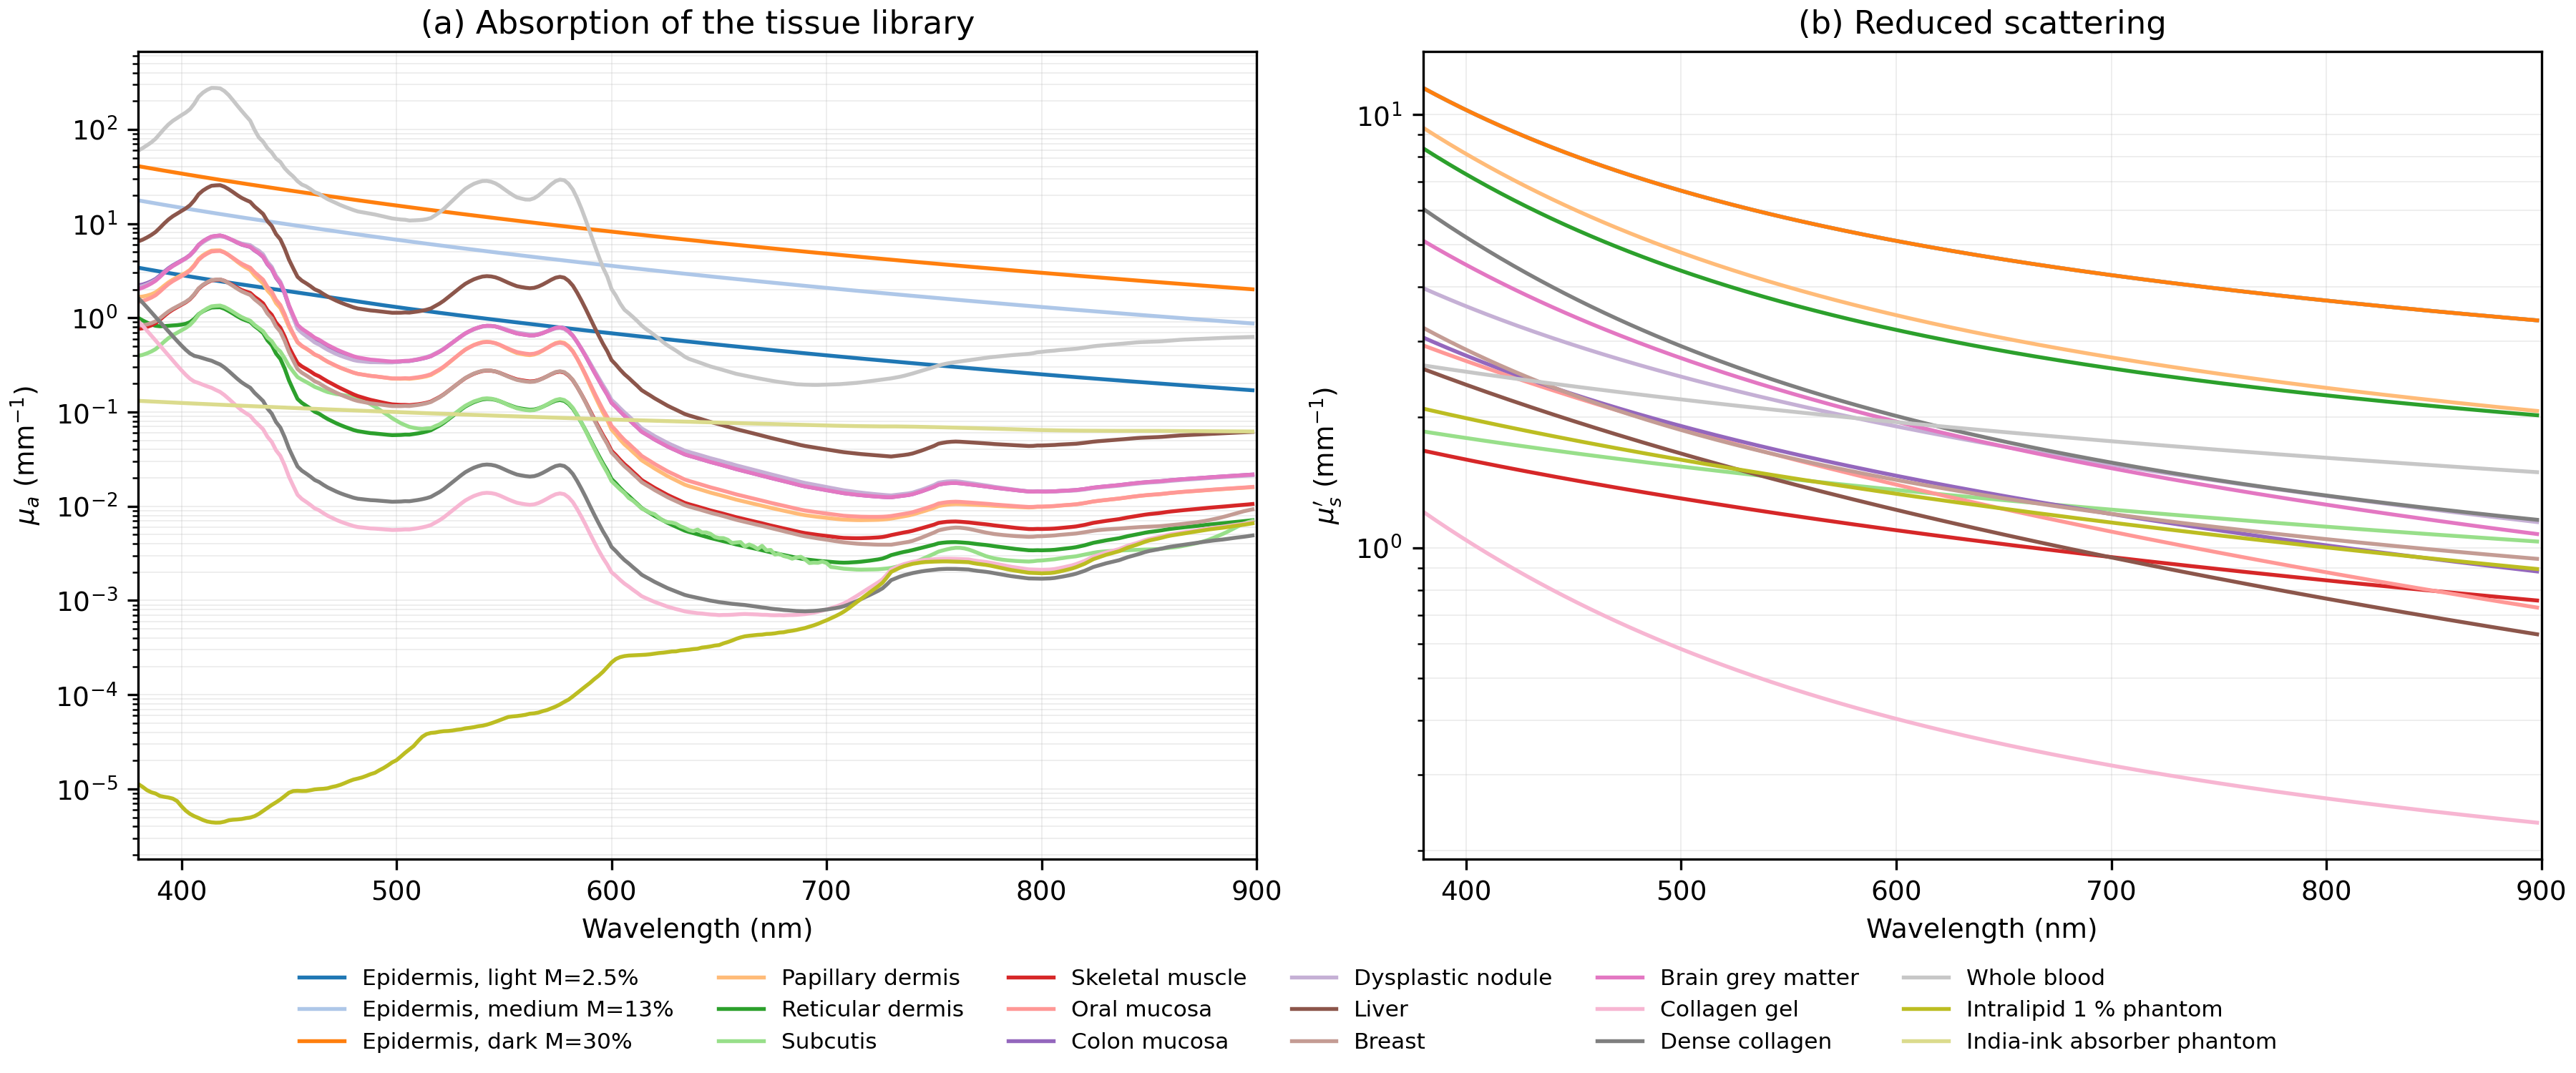
\includegraphics[width=0.92\textwidth]{fig21_tissue_optics.png}
\caption{Literature tissue-optics library: (a) absorption and (b) reduced scattering of the 18 materials, 380--900~nm.}
\label{fig:tissue}
\end{figure*}

\subsection{Layered-block 3D Monte Carlo}
\label{sec:mc3d}
A \emph{layered block} is a stack of layers whose interfaces are exact planes $y=a_i+b_ix+c_iz$ (uniform or linear-wedge thickness) bounded by four vertical faces and the bottom $y=0$, with air outside. Packets carry power $w$ (mW) and, as in MCML~\cite{wang1995mcml}, undergo implicit capture $w\leftarrow w\mus/\mut$, Henyey--Greenstein scattering~\cite{henyey1941}, Russian roulette and unpolarised Fresnel reflection or refraction at the true plane normal, so a wedge steers light correctly and total internal reflection is included. The bottom face is a Fresnel interface to air: $w(1-R)$ leaves and is lost to the stage, $wR$ stays in the block. Absorption is tallied on a \emph{layer-conforming} voxel grid with lateral cells of size $\Delta$ and a fixed number of sublayers across the local thickness $t_l(x,z)$, so a voxel volume is $V_v=\Delta^2t_l/S$ (exact because $t_l$ is linear) and a zero-thickness wedge end is represented without staircasing.

\emph{Excitation pass.} Once per excitation line, packets are launched from a jittered grid on the faces that face the source with weight $S\cos\theta_{\rm inc}\,dA\,T_{\rm other}$ per mW. The specular part of the entry Fresnel split is not transported (the tracer renders it as glint). The pass tallies the track-length fluence
\begin{equation}
\Phi_v=\frac1{V_v}\sum_{\rm segments} w\,\ell,\qquad P_{{\rm abs},v}=\mua\Phi_vV_v,
\label{eq:fluence}
\end{equation}
and the energy balance $R+T+A+\text{specular}+\text{lost}=1$. The absorbed power of a layer is split between its dyes in proportion $\mua^{(d)}/\mua^{\rm tot}$; each channel (excitation, layer, dye) becomes an emission source $A_d\,\Phi_d^{\rm eff}\,s\,(1-E_{\rm FRET})$, plus a Raman channel in aqueous layers.

\emph{Emission pass.} Once per emission wavelength node, source voxels are drawn by stratified inverse-CDF sampling on the total source $q(v)=\sum_c\sigma_{c,v}$, uniformly inside the voxel and with isotropic direction. A packet carries $\mathrm{coef}_c=\sigma_{c,v}\,Q/(q(v)N)$, so a single run serves all channels of all excitations; the radiance tally is then multiplied by the area-normalised emission density $e_c(\lem)$. Nodes are placed adaptively (dense where the transport factor bends) and the factor is interpolated linearly between them, since the sharp structure lives in $e_c$.

\emph{Cone estimator and peel-off.} Counting only packets that leave inside the camera cone of half-angle $\theta_a$ gives the unbiased estimate
\begin{equation}
L_{\rm cell}=\frac{\sum_{\rm cone}w}{A_{\rm cell}\,(\mathbf n\!\cdot\!\mathbf c)\,\pi\sin^2\theta_a},
\label{eq:cone}
\end{equation}
which is noisy for the small cells needed to resolve a wedge. The \emph{peel-off} (next-event) estimator instead adds, at every scattering event and at the launch of an emission packet, the expected contribution of the straight line of sight to the camera. The internal direction $\mathbf d$ follows from inverting Snell's law through the interface chain, and
\begin{equation}
\begin{split}\delta L_{\rm cell}&=\frac{w\,p_{\rm HG}(\mathbf u\!\cdot\!\mathbf d)\,T\,e^{-\tau}J}{A_{\rm cell}(\mathbf n\!\cdot\!\mathbf c)}\,\omega_{\rm MIS},\\ J&=\prod_j\frac{n_{{\rm up},j}^2\cos\vartheta_{{\rm up},j}}{n_{{\rm in},j}^2\cos\vartheta_{{\rm in},j}},\end{split}
\label{eq:peel}
\end{equation}
where $\tau$ is the optical depth of the straight segments, $T$ the product of Fresnel transmittances, $J$ the \'etendue factor that converts solid angle inside to solid angle in air, and $\omega_{\rm MIS}=1/(1+\Omega_c\,p\,J)$ a balance-heuristic multiple-importance weight~\cite{veach1995} that bounds the forward-peaked tail of the phase function ($\Omega_c$ the cone solid angle). A flag marks the paths the peel-off does not cover (the launch and the path after a Fresnel reflection), which the cone estimator still scores, so nothing is counted twice; side faces use the cone estimator. The peel-off needs about five times fewer packets (photon counts are scaled by 0.2), and the top-face tally is smoothed with a sub-cell Gaussian of $\sigma=0.35$~mm.

\emph{Determinism.} Photons are cut into fixed batches that re-seed from (seed, batch) and own private tallies summed in batch order, so results are bit-identical for any thread count.

\subsection{Inclusions}
\label{sec:inclusions}
A layered block may embed spheres, ellipsoids, cylinders and boxes (vessels are cylinders). The layer planes stay exact; the inclusions live on a regular Cartesian voxel map over the bounding box of the block, with voxel size $h$ (default $0.2$~mm), $2\times2\times2$ analytic supersamples per voxel and an integer region id ($0$ for the layer material, $r\ge1$ for inclusion $r$). A later inclusion wins overlaps; a mixed voxel takes the majority id among its in-block samples (ties go to the inclusion) and is optically homogeneous; inclusions are index-matched to the host, so there is no Fresnel boundary at their surface. The photon step is limited by the layer planes and, inside 4$^3$-voxel coarse zones that contain an inclusion voxel, by voxel boundaries; the dimensionless free path is carried across each partial move, so a change of $\mut$ at a boundary is exact. Voxel crossings consume no random number and the roulette is not rolled after them, so an inclusion with the host's optics follows the host-only random walk. Host and inclusion tallies are kept separate and together conserve the absorbed power. Inclusions can carry dyes and emit; emission sources inside them are sampled from the inclusion voxels. Each capture returns ground truth per inclusion: a mask, the depth of the inclusion below the surface, the fraction of the pixel's fluorescence that originates in it, and an \emph{Explain pixel} component per (dye, inclusion). A block without inclusions takes exactly the earlier code path and its results are bit-identical. With four inclusions occupying $1.4\,\%$ of the voxels the run time is about $2.0\times$ (excitation pass) and $2.1\times$ (emission pass) that of the homogeneous block, measured by interleaved runs on a loaded machine, so only the ratio is meaningful.

\subsection{Sensor, tunable-filter bands and noise}
The camera model follows a thin lens focused at distance $S$ with f-number $N$, transmission $T$, magnification $m$. For a pixel of area $A$ (including binning) exposed for $t$, the electrons collected in band $b$ are
\begin{equation}
\begin{split}e_b&=k_0\cos^4\!\theta\,A\,t\int L(\lambda)R_b(\lambda)\,T_{p,b}\,\mathrm{QE}(\lambda)\frac{\lambda}{hc}\,\mathrm d\lambda,\\ k_0&=\frac{\pi T}{4N^2(1+m)^2},\end{split}
\label{eq:electrons}
\end{equation}
with $R_b$ the band response (pass-band times long-pass edge) and $T_{p,b}$ the peak transmission. Liquid-crystal tunable filters (LCTF)~\cite{morris1994lctf} are Gaussian pass-bands, filter wheels super-Gaussian of order six; a ray at field angle $\theta$ sees the centre wavelength shifted to $\lambda_0\sqrt{1-\sin^2\theta/n_{\rm eff}^2}$, and the cube is resolved in six field-angle rings. Blur is the thin-lens circle of confusion with an Airy floor and axial chromatic shift, varying per pixel and band. The detector chain is
\begin{equation}
\begin{split}S\to S(1+\mathrm{PRNU})&\to+\text{dark}\to\mathrm{Poisson}\to+\mathcal N(0,\sigma_r^2)\\&\to\text{clip}\to\div g\to\text{round},\end{split}
\label{eq:detector}
\end{equation}
so for one pixel the variance in electrons squared is
\begin{equation}
\sigma^2(S)=(S+D)+\sigma_r^2+g^2/12,
\label{eq:variance}
\end{equation}
where $D$ is the dark signal and $g^2/12$ the quantisation noise~\cite{janesick2007,healey1994}; for the mean of an ROI with $n$ pixels it is divided by $n$. A white-reference mode renders a Spectralon plate with the same band set so that sample$/$white reproduces the laboratory normalisation, and a dark mode removes the source.

\section{Research Toolkit}
\label{sec:toolkit}
\subsection{Study engine and provenance}
A \texttt{StudySpec} names a base experiment (or preset), a list of parameters addressed by JSON pointers (continuous, integer or choice, linear or log scale, with optional linked pointers), a design (grid, random, Latin hypercube, Sobol' sequence, Saltelli or Morris), replicate seeds and metrics (ROI band sums and ratios, peak wavelength, EEM integral, Michelson or Weber contrast, contrast-to-noise ratio, ground-truth statistics). Each run is journaled so a study is resumable, every capture can embed its provenance, and a Methods-text generator produces a description of the experiment and study from the specification.

\subsection{Global sensitivity analysis}
For inputs scaled to the unit cube and a Saltelli design with matrices $A$, $B$ and $AB_i$ ($A$ with column $i$ from $B$) and $N$ base samples, the first-order and total effects are
\begin{align}
V_i&=\frac1N\sum_{j}f(B)_j\big[f(AB_i)_j-f(A)_j\big],\label{eq:Si}\\
V_{T_i}&=\frac1{2N}\sum_{j}\big[f(A)_j-f(AB_i)_j\big]^2,\label{eq:ST}
\end{align}
with $S_i=V_i/\mathrm{Var}(Y)$ and $S_{T_i}=V_{T_i}/\mathrm{Var}(Y)$ (estimators of Saltelli \emph{et al.}~\cite{saltelli2010} and Jansen~\cite{jansen1999}; Sobol' indices~\cite{sobol2001}). The first-order estimator is applied to outputs centred on $\tfrac12(\bar f(A)+\bar f(B))$ (recomputed inside each bootstrap resample): the estimator is unbiased either way, but its variance scales with the squared output mean, which for band signals far exceeds the spread, and an uncentred version returned $\sum_i S_i=-13$ for the peak wavelength in our data; $S_{T_i}$ is shift-invariant. Confidence intervals are percentile bootstraps over base rows. Morris screening~\cite{morris1991,campolongo2007} reports $\mu^*=\mathbb E|EE_i|$ and $\sigma=\mathrm{sd}(EE_i)$ of the elementary effects. With $R$ replicate seeds per design point, the within-point variance $s_w^2$ gives the Monte Carlo noise floor $(s_w^2/R)/\mathrm{Var}(\text{replicate means})$, the fraction of output variance that is engine noise; indices below it are not distinguishable from zero.

\subsection{Unmixing}
The joint EEM of a pixel (all bands of all excitations, $C$ channels) is modelled as $\mathbf y=\mathbf E\mathbf a+\boldsymbol\epsilon$, which is exact for independent emitters seen through the same optical path and approximate when the paths differ, which is precisely the cover effect studied here. Endmembers come from the forward model (the per-pixel component decomposition at the purest pixels, an in-silico equivalent of a pure-component capture through the same instrument), from user ROIs, or from NMF~\cite{lee1999} or VCA~\cite{nascimento2005}. Solvers are least squares, non-negative least squares~\cite{lawson1995} and fully constrained least squares ($a_k\ge0,\ \sum_ka_k=1$) by the augmented-NNLS construction of Heinz and Chang~\cite{heinz2001}, optionally with inverse Poisson--Gaussian channel weights.

\subsection{Surrogates and maximum-likelihood retrieval}
A surrogate replaces the Monte Carlo forward model by an interpolant $\mu_c(\boldsymbol\theta)$ of the noise-free ROI-mean signal of every channel on a grid or Sobol' set of one to three parameters. The noise-free output (expected electrons, before detector noise) is used, and the Monte Carlo seed is fixed across the grid (common random numbers) so finite-difference Jacobians are smooth; residual Monte Carlo noise is removed with a smoothing spline chosen by generalised cross-validation. The estimator minimises
\begin{equation}
\begin{split}\chi^2(\boldsymbol\theta)&=\sum_c\frac{[y_c-\mu_c(\boldsymbol\theta)]^2}{\sigma_c^2(\mu_c)},\\ \sigma_c^2&=\frac{(\mu_c+D_c)+\sigma_r^2+g^2/12}{n},\end{split}
\label{eq:chi2}
\end{equation}
by iteratively re-weighted trust-region least squares, with start points from a scan of a dense surrogate table so that non-monotonic signals do not depend on the user's guess. The fixed point solves the Gaussian maximum-likelihood and, for Poisson data, the Poisson likelihood estimating equation $\mathbf J^\top\mathbf W(\mathbf y-\boldsymbol\mu)=0$. Confidence intervals are profile-likelihood intervals~\cite{venzon1988}, $\{\theta_p:\min_{\rm others}\chi^2-\chi^2_{\min}\le q_{\chi^2}(\text{level},1)\}$, and open intervals are flagged. A map retrieval fits one parameter vector per tile of a noisy capture and reports bias, RMSE and interval coverage against the ground truth.

\subsection{Fisher information, CRLB and optimal design}
With channels independent and Poisson--Gaussian variance~\eqref{eq:variance}, the Fisher information is
\begin{equation}
\mathbf F=\sum_{c=1}^C \mathbf I_c,\qquad \mathbf I_c=\frac{\mathbf J_c\mathbf J_c^{\top}}{\sigma_c^2(\mu_c)},\quad J_{c,i}=\frac{\partial\mu_c}{\partial\theta_i},
\label{eq:fisher}
\end{equation}
and the Cram\'er--Rao bound on any unbiased estimator is $\mathrm{Cov}(\hat{\boldsymbol\theta})\succeq\mathbf F^{-1}$. Eq.~\eqref{eq:fisher} equals the Poisson information $\mu'^2/\mu$ when read noise vanishes and the Gaussian information when the signal is read-noise limited; the term from the dependence of the variance on $\boldsymbol\theta$ is neglected. The forward model is imperfect, so a purely photon-limited $\mathbf F^{-1}$ is optimistic. We therefore add a systematic model-error term to every channel,
\begin{equation}
\sigma_c^2\;\to\;\sigma_c^2+(\epsilon\,\mu_c)^2,
\label{eq:modelerr}
\end{equation}
with a relative error $\epsilon$ that we estimate from the sim-to-real residuals: the median relative RMS residual of the 22 calibrated fits (nine collagen ROIs, 16 droplets, \texttt{derive\_eps}) is $7.0\,\%$ (range $5.3$--$9.6\,\%$), an upper bound because it contains camera noise. The term acts as independent per-channel variance and is optimistic if real errors are correlated across channels; it also does not represent bias. Because $\mathbf F$ is a sum of per-channel matrices, choosing $k$ channels is the classical design problem~\cite{pukelsheim2006}. D-optimality maximises $\log\det\mathbf F$, A-optimality minimises $\tr\mathbf F^{-1}$, and the target (c-optimal) criterion minimises $[\mathbf F^{-1}]_{pp}$, the bound of one parameter. The first is monotone and submodular, so the greedy set is within $1-1/e$ of the optimum~\cite{nemhauser1978}; it is checked against exhaustive search when $\binom Ck$ is small. Exposure allocation over selected channels uses $I_c(t)=\mathbf J_c\mathbf J_c^\top(t/t_0)^2/\sigma_c^2(t)$ under a total-time budget and a full-well limit: it is convex in the shot-limited regime and solved by sequential quadratic programming otherwise. The selected set can be compared with the channels chosen by the label-free selectors of our earlier work~\cite{meloyan2025scirep}.

\subsection{Calibration and digital twin}
For an optically thin, dilute layer the electrons in band $b$ at excitation $\lex$ are
\begin{equation}
S[\lex,b]=\sum_ka_k\,A_k(\lex)\,M_k(\lex,b),
\label{eq:calib}
\end{equation}
with $A_k=\sum_\lambda \mathrm{line}_{\rm ex}(\lambda)\,\mathrm{exc}_k(\lambda)$ the excitation overlap, $M_k=\sum_\lambda R_b(\lambda)e_k(\lambda)$ the emission band projection and $a_k=c_k\varepsilon_k\Phi_k\ln10/10$ a lumped amplitude that cannot be separated into concentration, extinction and yield from relative data. Gains (a global scale, or one scale per excitation) are eliminated in closed form by variable projection~\cite{golub1973}, so the optimiser sees only shape parameters (excitation and emission peak and width, red-tail skew, vibronic shoulder). The objective is a robust soft-L1 loss of per-excitation relative residuals from deterministic multi-starts; covariance is $s^2(\mathbf J^\top\mathbf J)^+$ (statistical only), and a pixel bootstrap is available. Optional shared instrument terms are a smooth log-throughput polynomial and an LCTF ripple orthogonal to cubic polynomials. Which parameters are identifiable is reported explicitly, e.g. an emission peak below the first band is not.

\section{Validation}
\label{sec:validation}
All numbers below are regenerated by scripts in the repository; only literature reference values are hard-coded. Table~\ref{tab:valid} summarises the checks; the following subsections give details.

\begin{table*}[!t]
\caption{Summary of validation checks (engine versus analytic or independent reference).}
\label{tab:valid}
\centering\small
\begin{tabular}{@{}llll@{}}
\toprule
Check & Reference & Result & Section\\
\midrule
Wang--Jacques slab, $R_d$, $T_t$ & $0.09734$, $0.66096$ & $<0.1\,\%$ deviation & \ref{sec:v_mc}\\
Energy conservation (1D and 3D MC) & $R+T+A+\ldots=1$ & $10^{-9}$ & \ref{sec:v_mc}, \ref{sec:v_3d}\\
Clear index-mismatched slab & exact incoherent solution & $0.01\,\%$ & \ref{sec:v_mc}\\
Diffusion decay, $\mu_{\rm eff}$ & $0.1741$~mm$^{-1}$ & $0.1736$~mm$^{-1}$ ($-0.29\,\%$) & \ref{sec:v_mc}\\
Closed form vs.\ volume quadrature & internal & $0.008\,\%$ & \ref{sec:v_opt}\\
Dilute limit vs.\ legacy engine & ratio CV & $0.09\,\%$ & \ref{sec:v_opt}\\
Photon transfer: gain, read noise & $1.5$~e$^-$/ADU, $8.0$~e$^-$ & $1.501$, $7.99$ & \ref{sec:v_opt}\\
3D MC vs.\ MCML (benchmark slab) & MCML & $R$ $-0.21\,\%$, $T$ $+0.04\,\%$ & \ref{sec:v_3d}\\
3D bottom boundary, clear slab & closed form & agreement to 5 digits & \ref{sec:v_3d}\\
Peel-off vs.\ cone & cone estimator & $0.993$--$1.010$ & \ref{sec:v_3d}\\
Radial $R(\rho)$, 3D engine & independent MCML-type MC & within $1.1\,\%$ & \ref{sec:v_incl}\\
Null / filling inclusion & host-only run & identical (bit level, peel-off off) & \ref{sec:v_incl}\\
Absorbing sphere, $\Delta R$ & first-order perturbation theory & $0.948$ of prediction & \ref{sec:v_incl}\\
Twin fast model vs.\ full capture & full engine & $4.1\cdot10^{-4}$ max.\ rel.\ dev. & \ref{sec:v_s2r}\\
\bottomrule
\end{tabular}
\end{table*}

\subsection{Monte Carlo transport against standard benchmarks}
\label{sec:v_mc}
The baked white-Monte-Carlo tables and a conventional MCML implementation both reproduce the Wang--Jacques/Prahl slab benchmark ($\mua=1$, $\mus=9$~mm$^{-1}$, $g=0.75$, $n=1$, $d=0.2$~mm; $R_d=0.09734$, $T_t=0.66096$) to better than $0.1\,\%$ (Fig.~\ref{fig:mcml}), conserve energy to $10^{-9}$, match the exact incoherent multiple-reflection solution for a non-scattering, index-mismatched slab to $0.01\,\%$ and agree with each other for an oblique, index-mismatched turbid slab to $\le0.05\,\%$. Semi-infinite diffuse reflectance agrees with the Farrell--Patterson albedo formula~\cite{farrell1992} to $0.3\,\%$ ($n=1$) and $1.1\,\%$ ($n=1.4$; the dipole formula itself is good to a few percent at an index step). For a high-albedo medium ($\mua=0.01$, $\musp=1$~mm$^{-1}$, $g=0.9$) the absorbed-weight profile decays as $\exp(-\mu_{\rm eff}z)$ with a fitted $\mu_{\rm eff}=0.1736$~mm$^{-1}$ against $\sqrt{3\mua(\mua+\musp)}=0.1741$~mm$^{-1}$ ($-0.29\,\%$) over nine decades~\cite{patterson1989}.

\begin{figure}[!t]
\centering
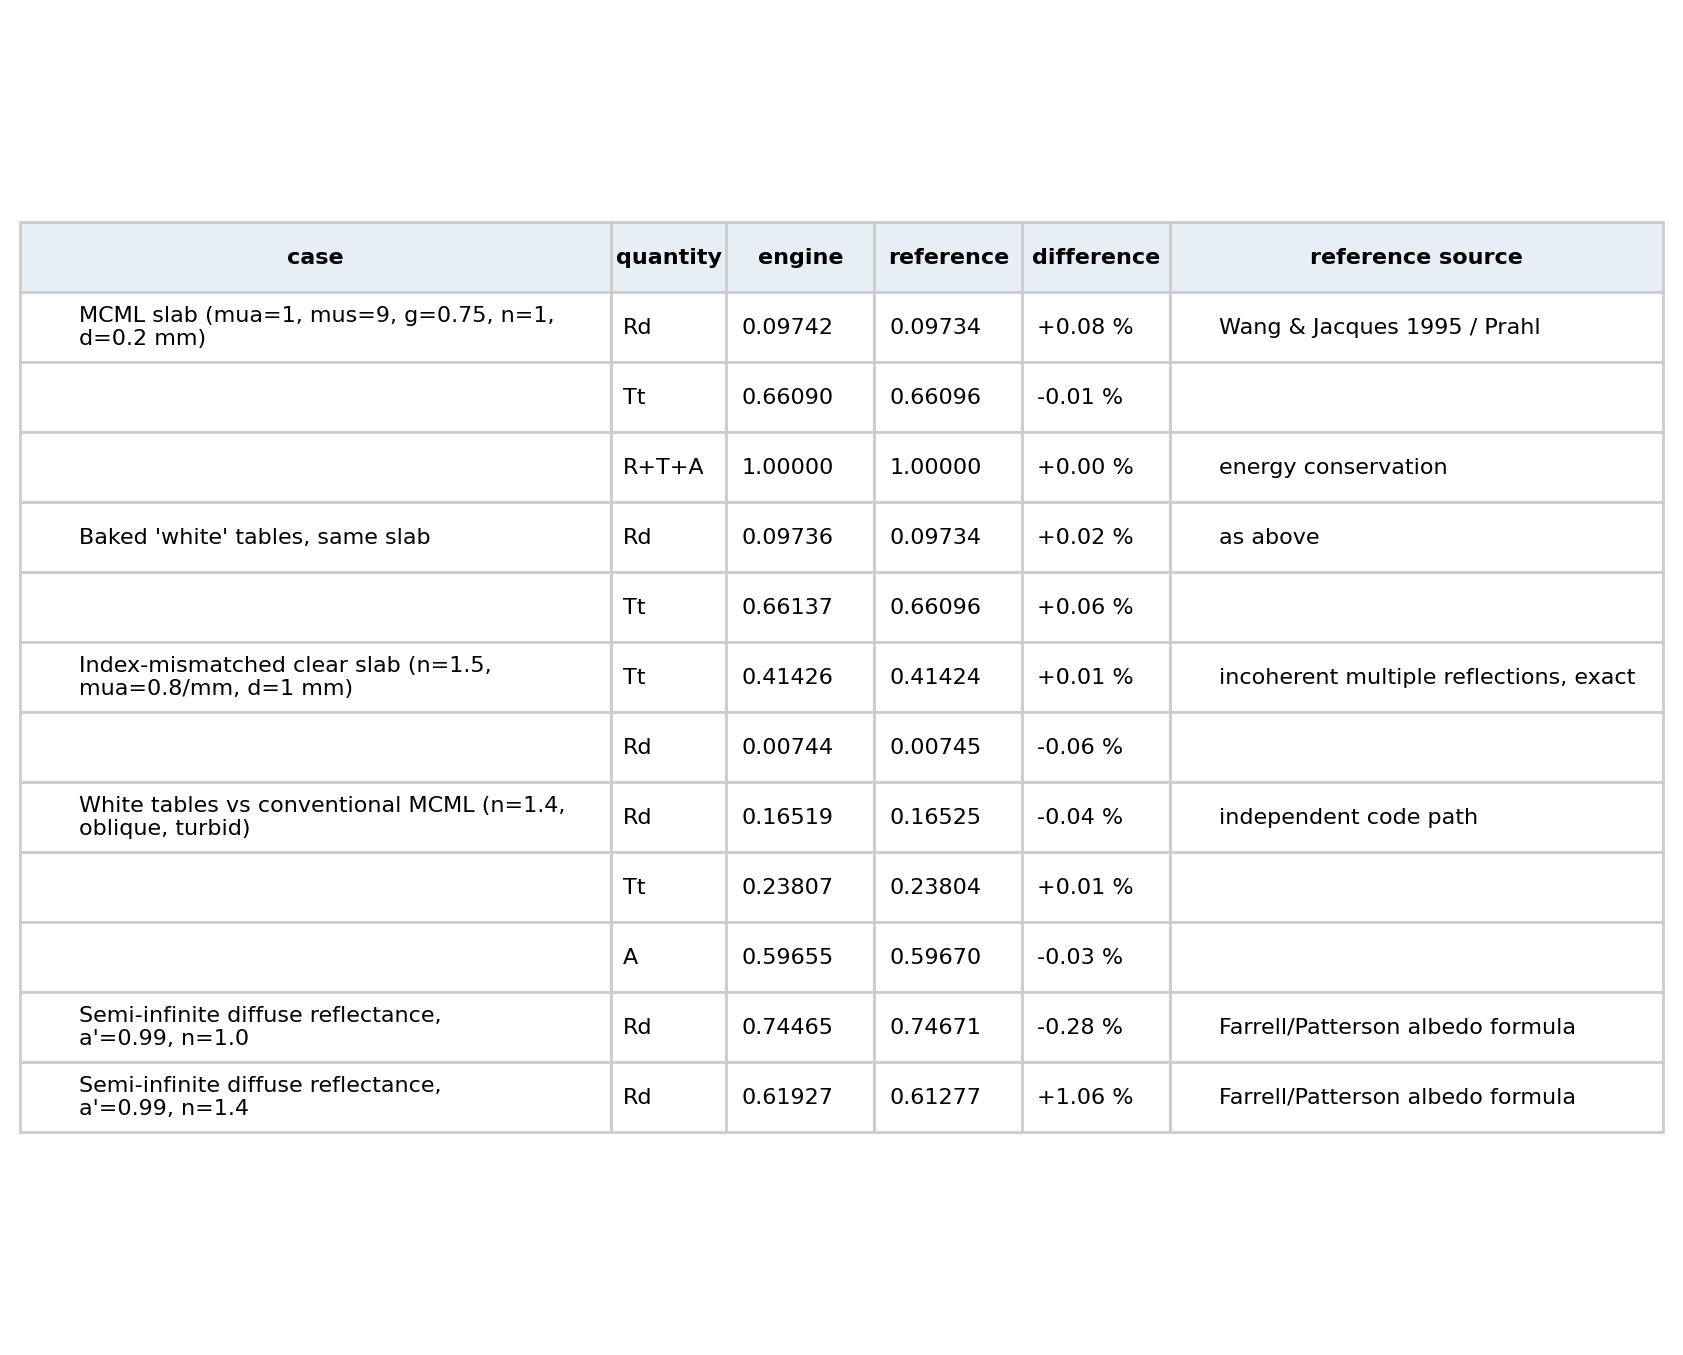
\includegraphics[width=\columnwidth]{fig01_mcml_table.png}
\caption{Baked Monte Carlo tables and a conventional MCML code against the Wang--Jacques slab benchmark~\cite{wang1995mcml}.}
\label{fig:mcml}
\end{figure}

\subsection{Optics, photophysics and sensor}
\label{sec:v_opt}
Two independent implementations of the clear-medium physics, the closed form of Eq.~\eqref{eq:Gclear} and the per-pixel volume quadrature, agree to $0.008\,\%$ from $0.1$~\textmu M to 1~mM fluorescein for a laterally uniform beam. In the dilute limit the 3D engine and the legacy 2D engine give the same emission shapes and cross-excitation ratios up to one geometry constant (61 points; coefficient of variation $0.09\,\%$). The inner-filter effect behaves as expected~\cite{kubista1994} (Fig.~\ref{fig:inner}): in front-face geometry the signal per unit concentration saturates, while in 90$^\circ$ geometry the cuvette-integrated signal peaks near 13~\textmu M ($A_{1\,\rm cm}\approx0.9$) and the centre-pixel signal falls as $10^{-A/2}$. Reabsorption shifts the apparent fluorescein maximum from 512~nm (dilute) to 540~nm at 500~\textmu M across 9~mm of liquid, but only to 518~nm in the front-face slab. Photobleaching follows $\exp(-kn)$ with $k=0.094$ per step in a worked case, and the same total dose delivered as 300$\to$40~mW or 40$\to$300~mW records 76/55\,\% versus 96/71\,\% of the un-bleached signals. The photon-transfer curve of the detector chain returns the configured gain ($1.501$ against $1.5$~e$^-$/ADU) and read noise ($7.99$ against $8.0$~e$^-$) within $0.2\,\%$ and $0.1\,\%$. The depth-of-field blur coincides with the analytic thin-lens circle of confusion, and a 600~nm band shifts by $-1.5$~nm at the corner of the lab-replica field ($\theta_{\max}=8^\circ$, $-13$~nm at $25^\circ$).

\begin{figure}[!t]
\centering
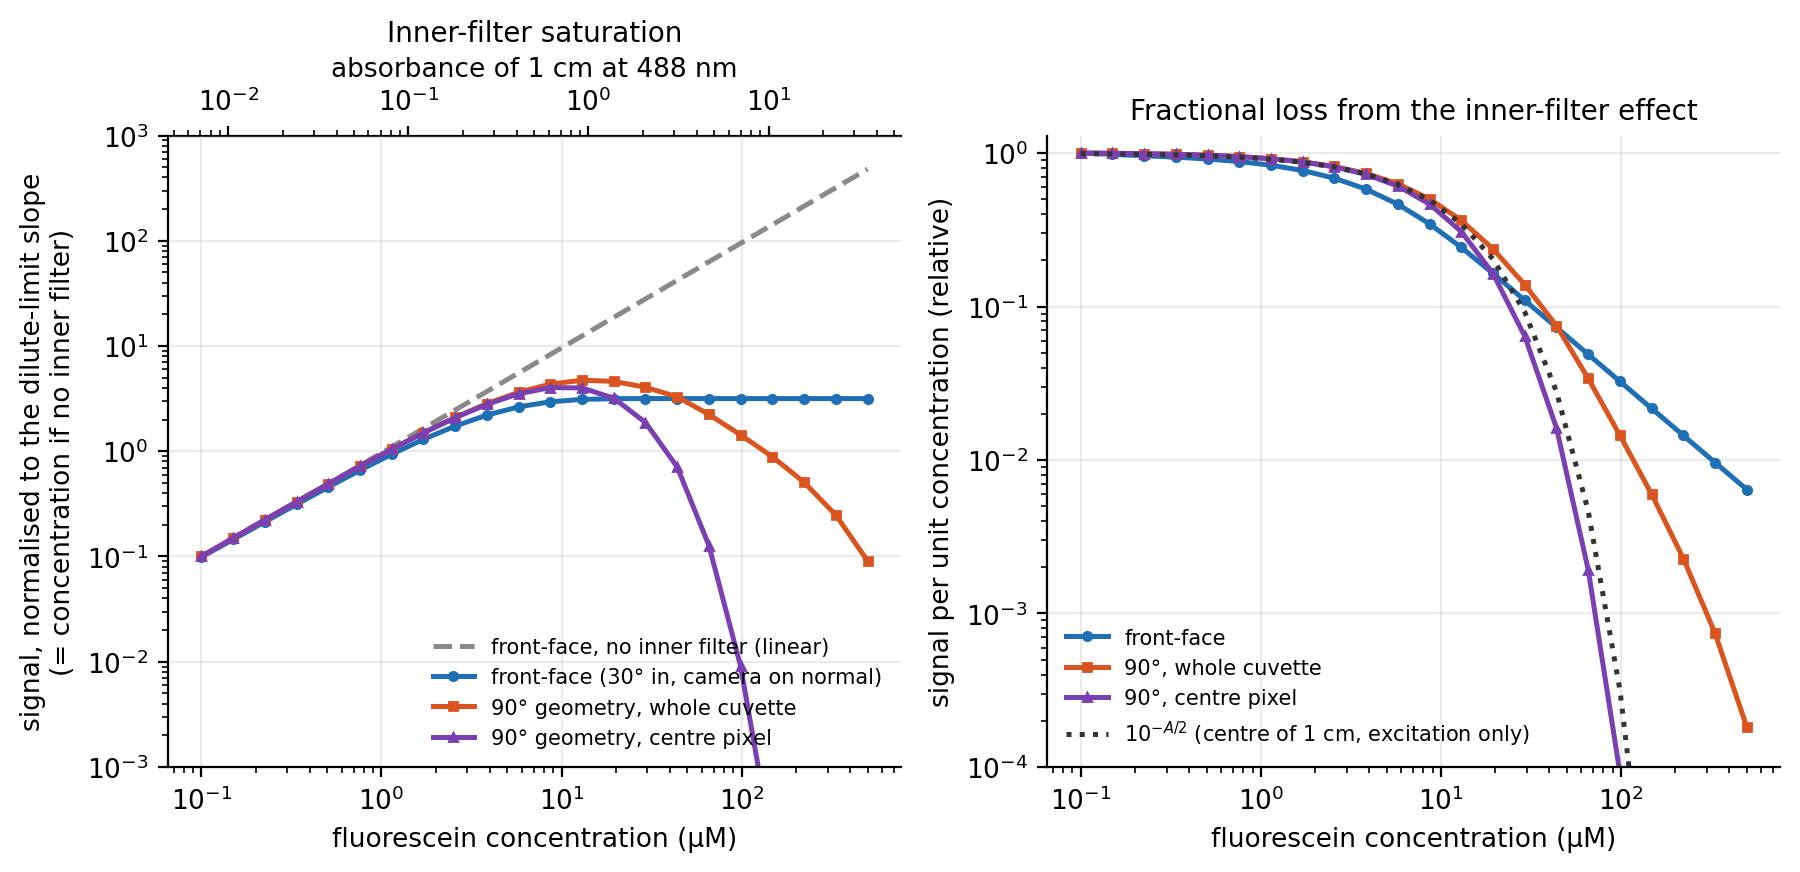
\includegraphics[width=\columnwidth]{fig05_inner_filter.png}
\caption{Inner-filter effect for fluorescein excited at 488~nm: front-face versus 90$^\circ$ geometry. The dotted curve is the excitation-only prediction $10^{-A/2}$ for the cell centre.}
\label{fig:inner}
\end{figure}

\subsection{Layered-block 3D Monte Carlo}
\label{sec:v_3d}
Homogeneous slabs reproduce the MCML implementation to Monte Carlo noise (benchmark slab $R$ $-0.21\,\%$, $T$ $+0.04\,\%$; index-mismatched slab $R$ $-0.05\,\%$, $T$ $+0.07\,\%$; tissue-like slab $R$ $-0.55\,\%$, $T$ $+0.98\,\%$, $A$ $-0.54\,\%$), energy is conserved to $10^{-9}$, and two identical stacked layers equal one layer of the summed thickness ($R$ $-0.04\,\%$, $T$ $-0.11\,\%$). A 2~mm fluorescent layer reproduces the 1D kernel result of Eq.~\eqref{eq:radiance} to $+0.14\,\%$ for fluorescence and $-4.04\,\%$ for elastic remission (Fig.~\ref{fig:blkref}). For clear slabs the bottom-boundary treatment matches the closed forms $T=(1-R_0)^2e^{-\tau}/(1-R_0^2e^{-2\tau})$ and $R_{\rm top}=(1-R_0)^2R_0e^{-2\tau}/(1-R_0^2e^{-2\tau})$ to the digits reported (e.g.\ $n=1.5$, $\mua d=0.5$: $T_{\rm bottom}=0.55931$ for both). Turbid fluorescent slabs captured as a block and as a 1D box (secondary emission off) agree: block$/$1D $=0.982$ at 6~mm and $0.987$ at 1~mm. Thick slabs (about 20~mm) differ by up to $20\,\%$ in the red tail for a physical reason: the 1D engine assumes laterally uniform irradiance while the block sees the finite lamp spot.

The peel-off estimator agrees with the cone estimator within $0.993$--$1.010$ across four configurations (Fig.~\ref{fig:peel}); at equal photon count the cell-to-cell standard deviation of a uniform field is reduced by a factor $3.7$ at $10^5$ photons and $2.0$ at $3\cdot10^6$ photons (about $6\times$ for $g=0$ and $2\times$ for $g=0.9$), and a sub-cell smoothing of $0.35$~mm reaches the noise level of the old cone estimator with five times fewer photons. For a buried fluorescein layer under a wedge cover the signal per unit surface irradiance falls roughly exponentially with local thickness (effective attenuation $0.43$~mm$^{-1}$ at 490~nm excitation) and the blue/red emission ratio stays within $1.78$--$1.83$, i.e.\ this nearly neutral cover attenuates but does not distort (Fig.~\ref{fig:wedge}). Under collagen (tissue with NADH/FAD at 365~nm), the buried signal drops by more than an order of magnitude between 0.2 and about 1~mm and the 440~nm band falls less than the 520~nm band, and the cover's own autofluorescence saturates with a decay length of $0.37$~mm (Fig.~\ref{fig:collagen}).

\begin{figure*}[!t]
\centering
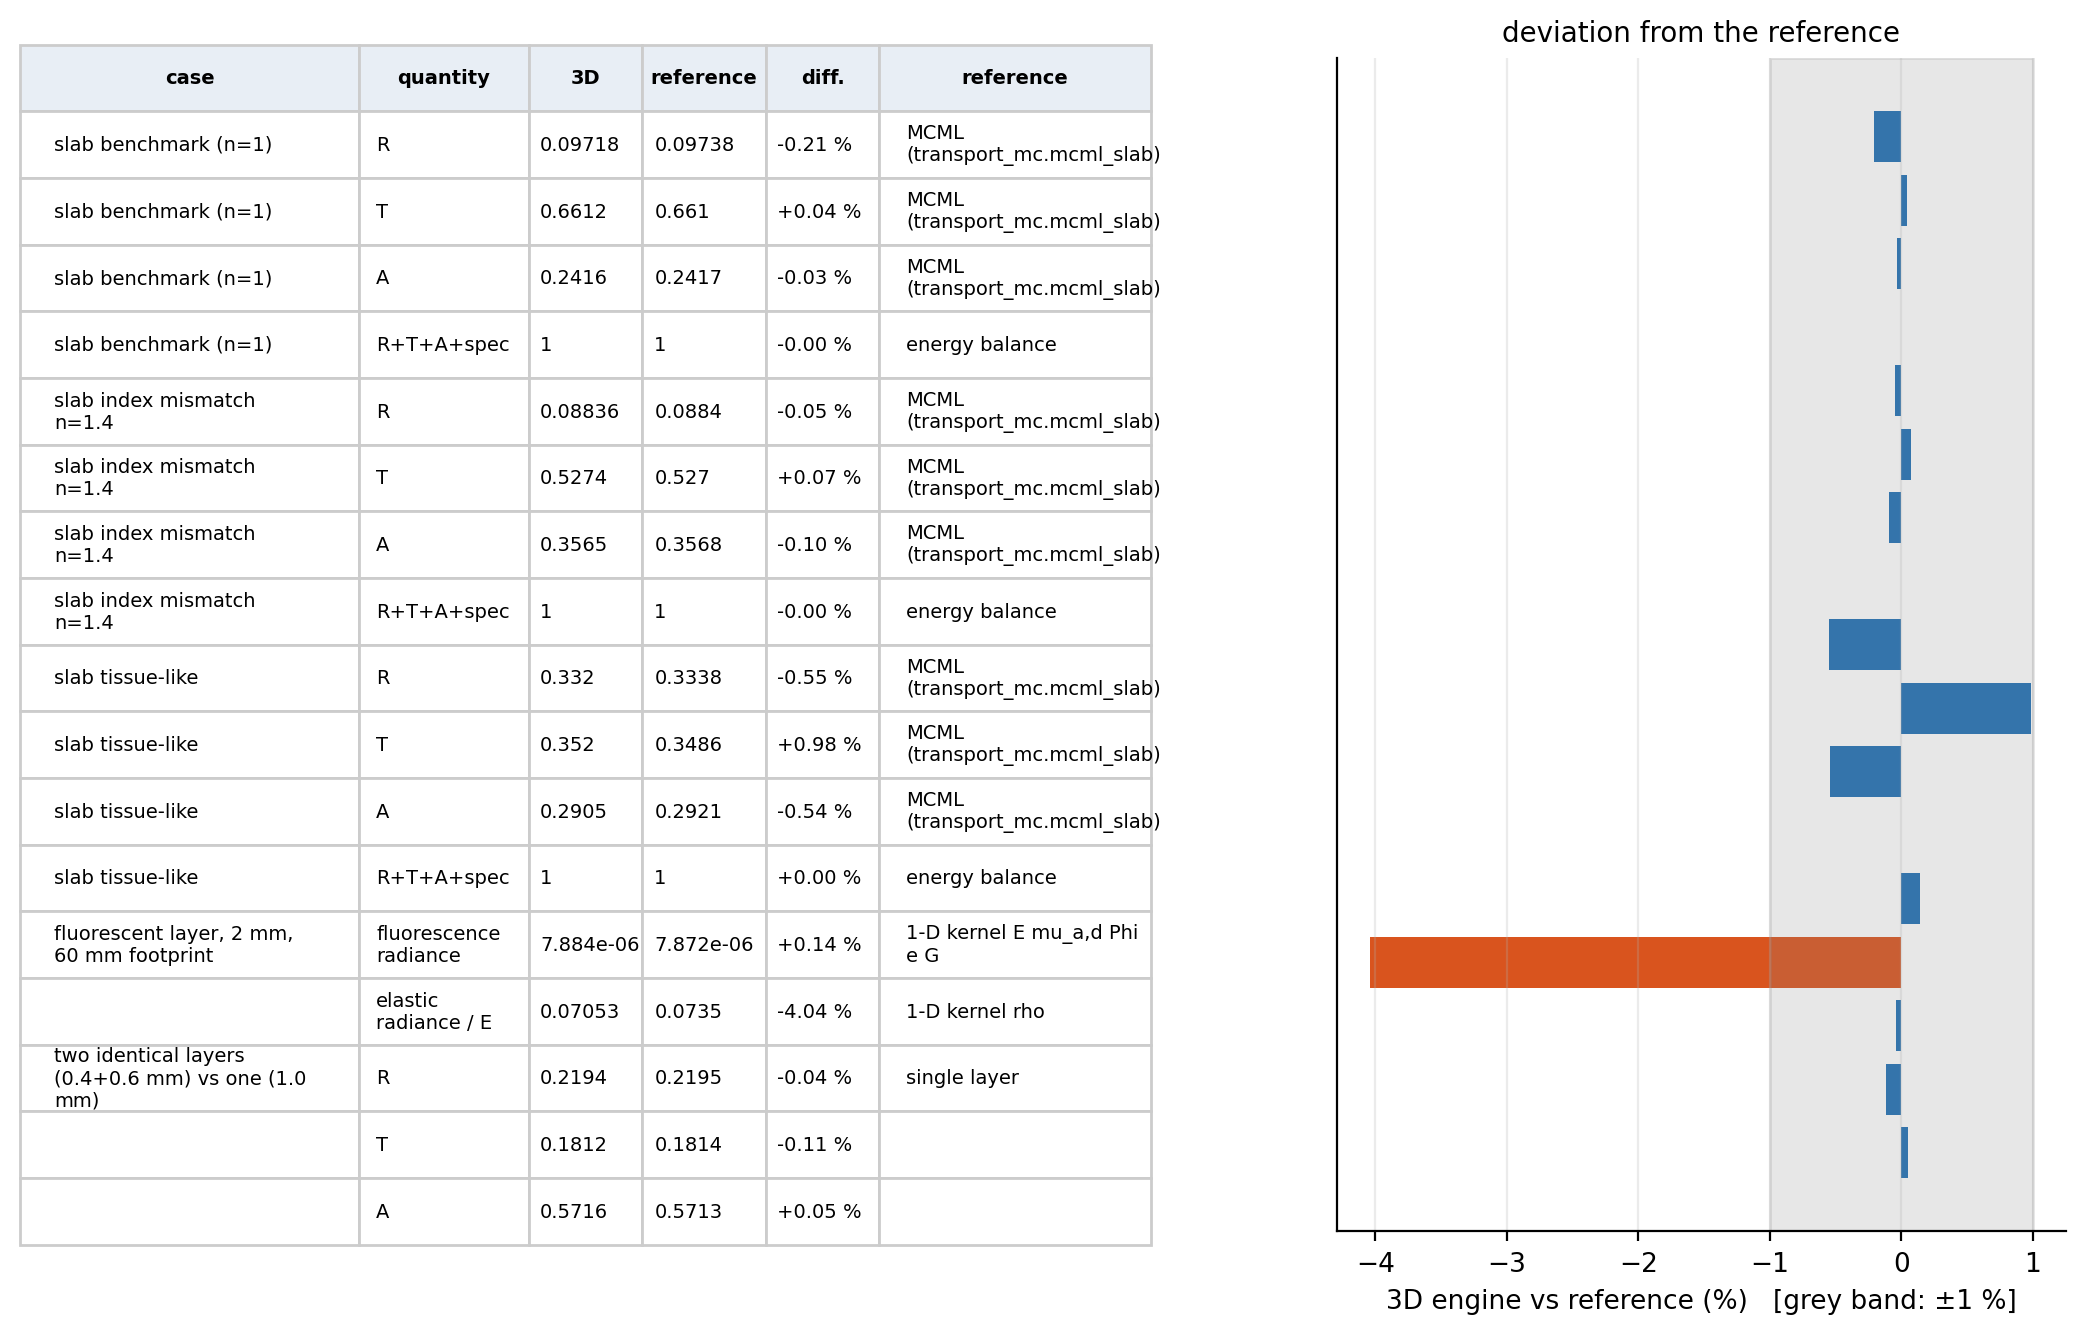
\includegraphics[width=0.92\textwidth]{fig12_blk_3d_vs_reference.png}
\caption{The 3D Monte Carlo against the MCML implementation and the 1D engine for homogeneous slabs and a fluorescent layer.}
\label{fig:blkref}
\end{figure*}
\begin{figure*}[!t]
\centering
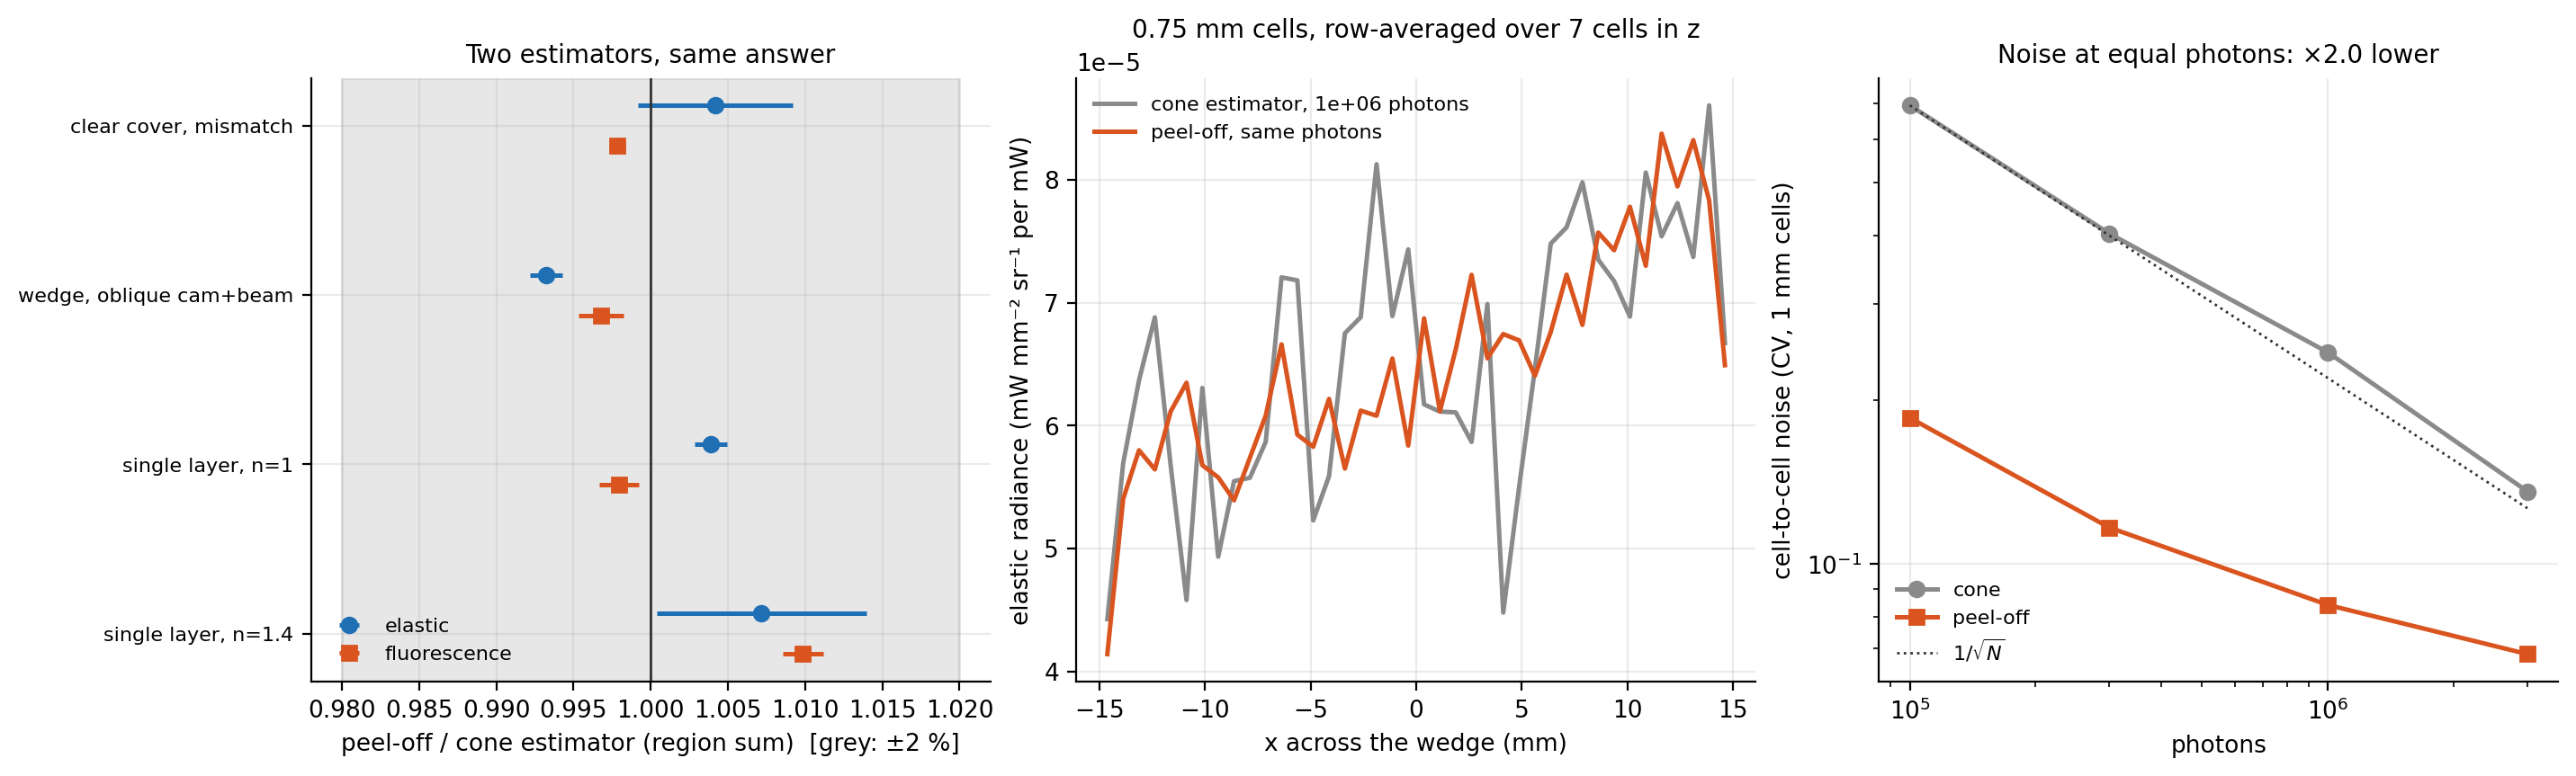
\includegraphics[width=0.92\textwidth]{fig14_blk_peel_vs_cone.png}
\caption{Peel-off versus acceptance-cone estimator: agreement of region sums and noise reduction at equal photon count.}
\label{fig:peel}
\end{figure*}
\begin{figure*}[!t]
\centering
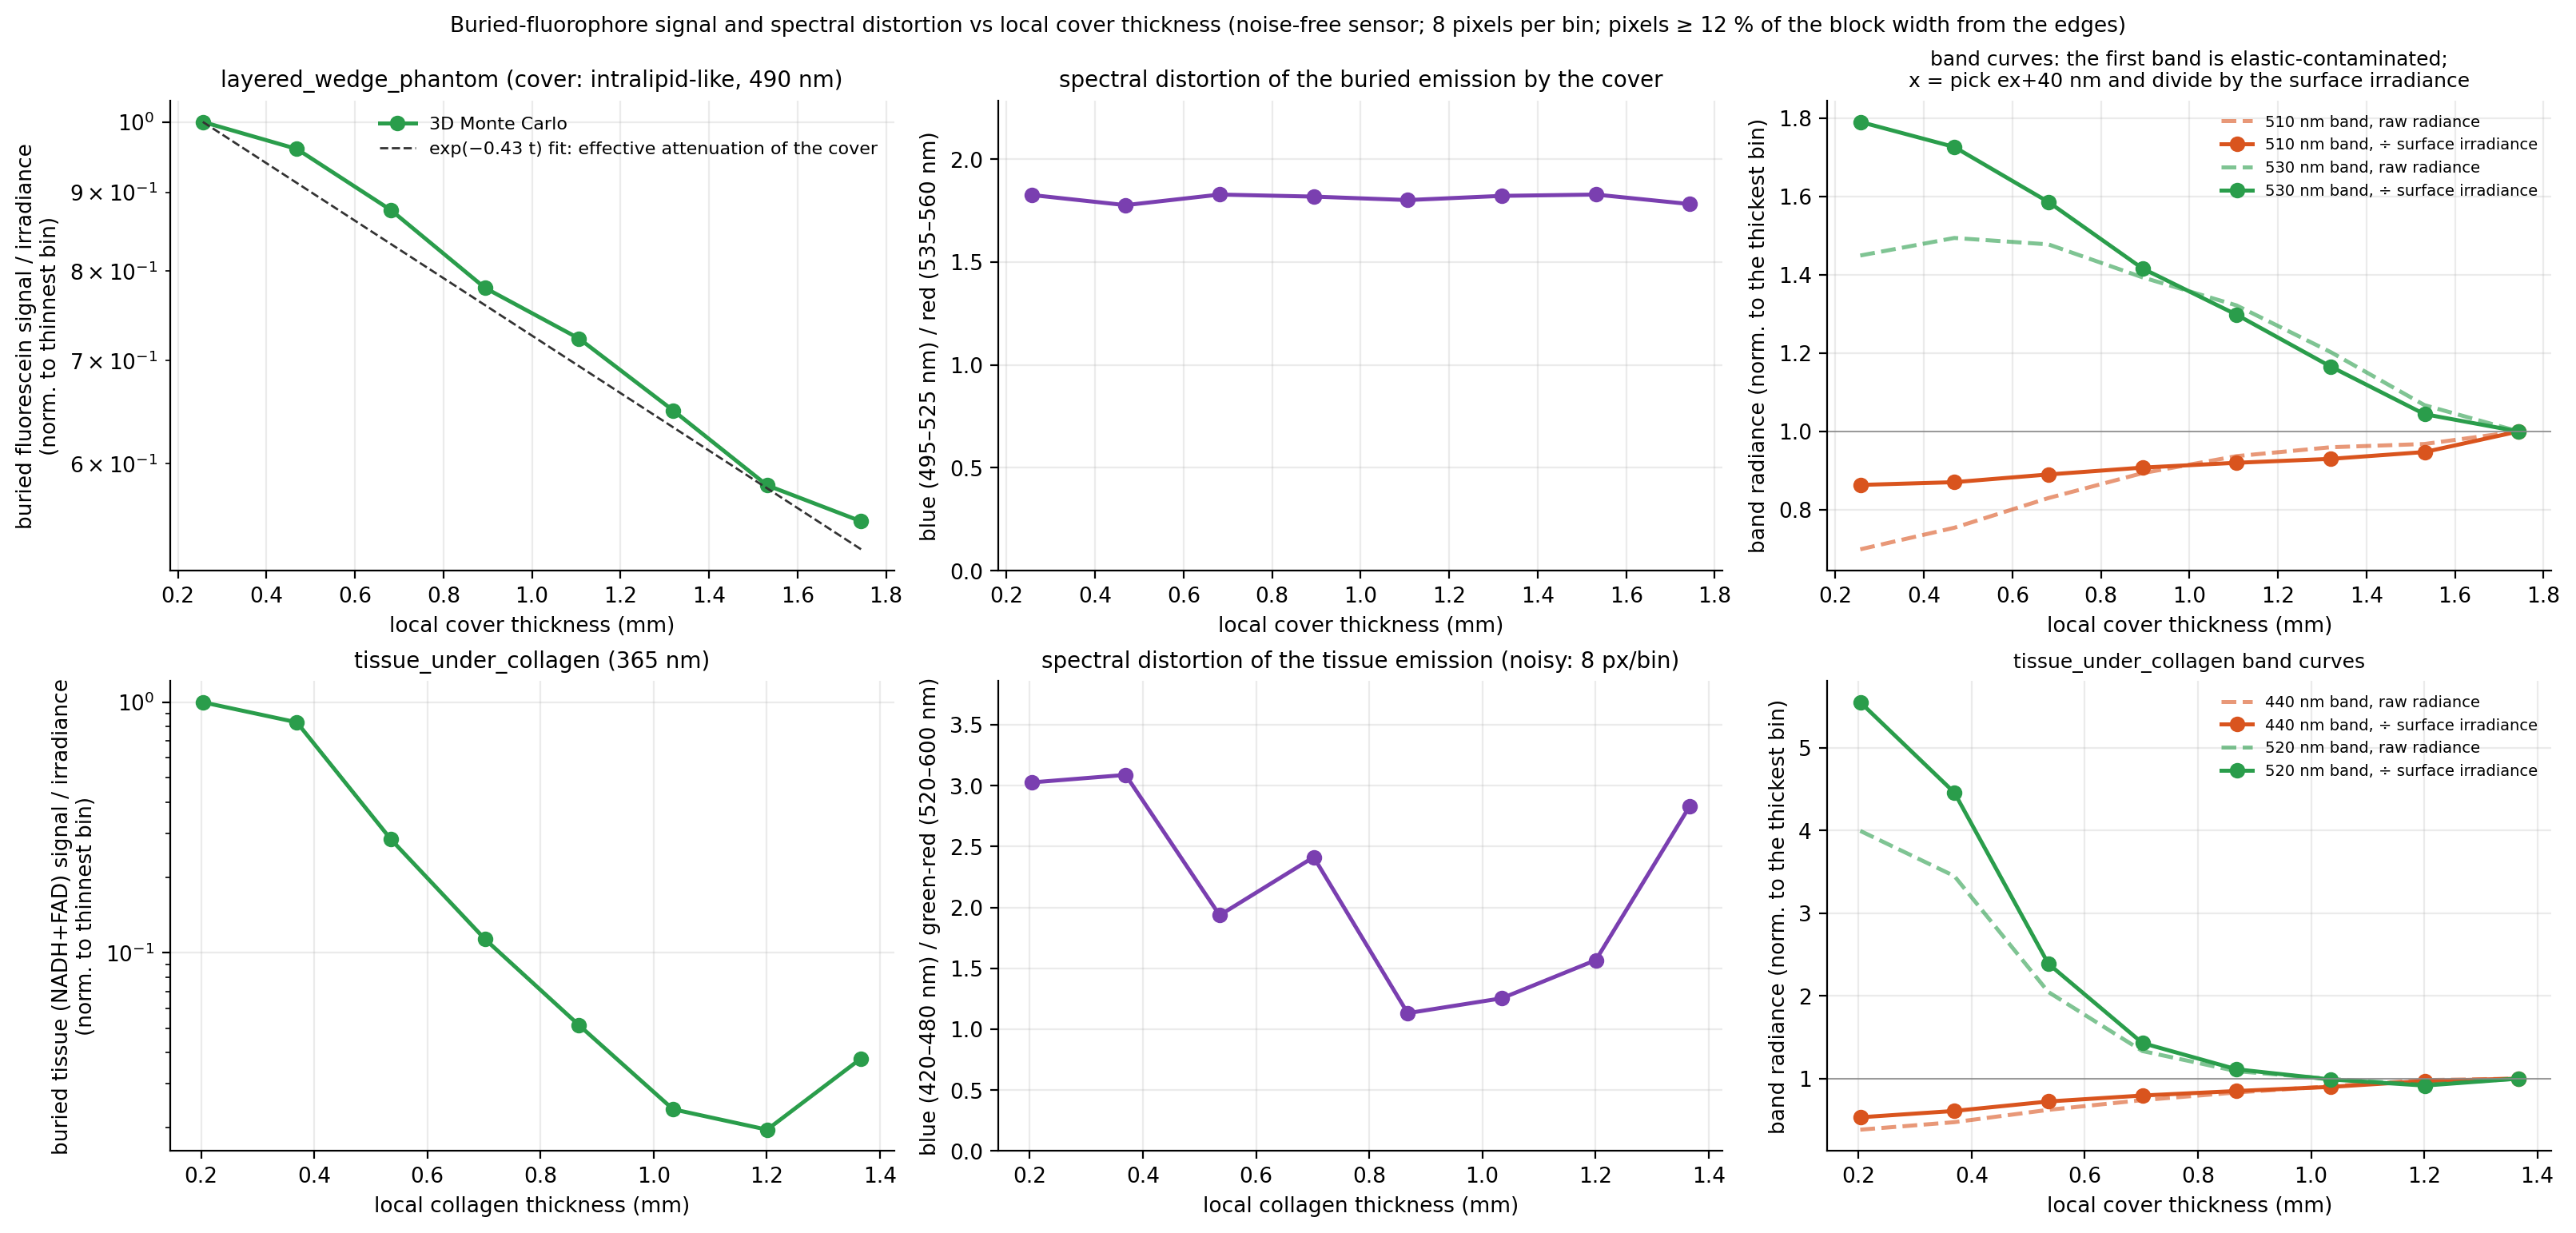
\includegraphics[width=0.92\textwidth]{fig15_blk_wedge_response.png}
\caption{Buried fluorophore under a wedge cover: signal against local cover thickness, and band ratios for a nearly neutral cover and for tissue under collagen.}
\label{fig:wedge}
\end{figure*}
\begin{figure*}[!t]
\centering
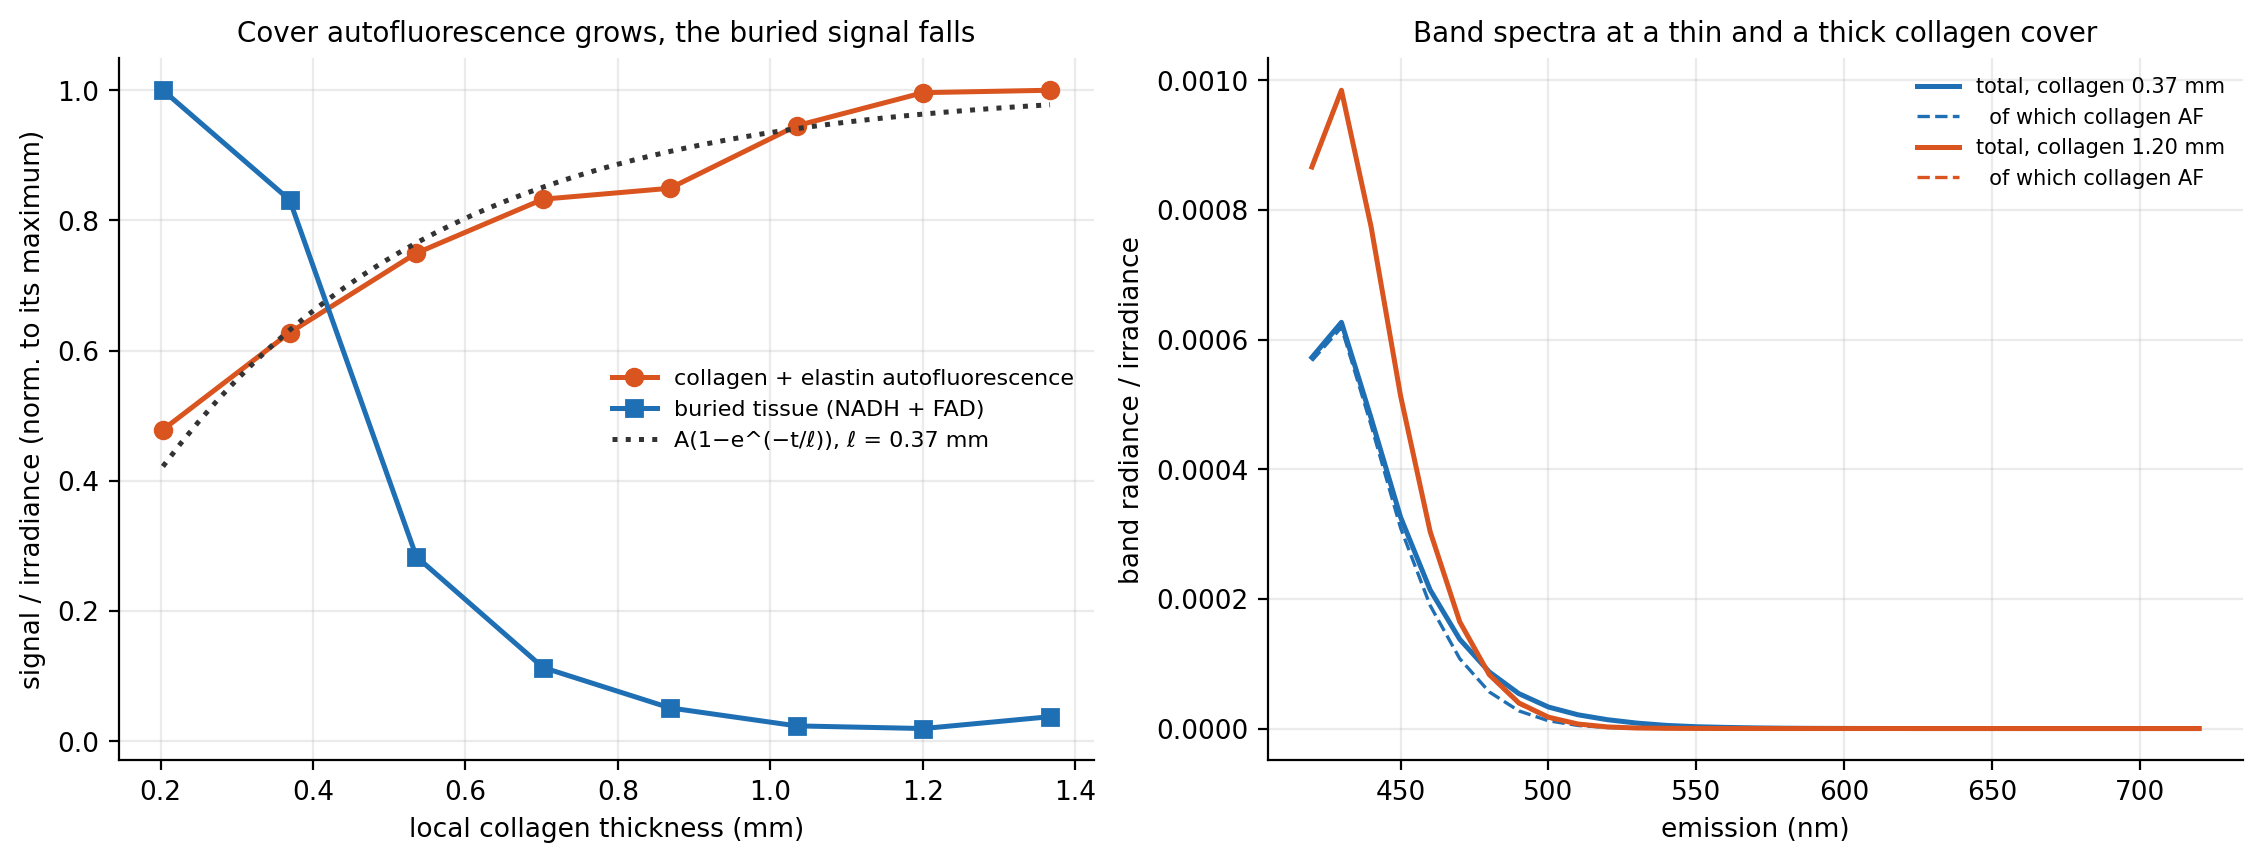
\includegraphics[width=0.92\textwidth]{fig17_blk_collagen_autofluorescence.png}
\caption{Collagen cover autofluorescence against thickness (saturating with decay length $0.37$~mm) while the buried NADH/FAD signal falls.}
\label{fig:collagen}
\end{figure*}

\subsection{Voxel inclusions and lateral transport}
\label{sec:v_incl}
\emph{Identities.} A null inclusion (same optics as the host) reproduces $R$, $T$ and $A$ of the host-only run to the last bit with the peel-off off ($2\cdot10^5$ photons), and the camera radiance to $6\cdot10^{-16}$ with it on. A box that fills a wedge layer equals replacing the layer, again to the last bit without peel-off; with peel-off on, $R$ differs by $0.19\,\%$ ($0.161004$ against $0.161303$), the camera radiance by $0.12\,\%$ and the layer absorption by $0.07\,\%$. $R+T+A+\text{specular}=1$ to better than $10^{-9}$ in all six test scenes (edge-straddling, wedge-crossing, clear, vessel with box), and the results are bit-identical for 1, 4 and 14 threads.

\emph{Lateral transport.} For a pencil beam on a semi-infinite block ($\mua=0.01$, $\musp=1$~mm$^{-1}$, $g=0$, $n=1.4$) the radial diffuse reflectance $R(\rho)$ of the 3D engine ($4\cdot10^6$ photons) agrees with an independent MCML-type code ($2\cdot10^7$ photons, no shared code) to within $1.1\,\%$ in all eight annuli between 1 and 10~mm (ratio $0.989$--$1.000$; statistical noise about $0.5\,\%$; total diffuse reflectance $0.6046$; Fig.~\ref{fig:radial}). Against the Farrell--Patterson--Wilson dipole~\cite{farrell1992} the engine is $-28\,\%$ at 1--1.5~mm, $+0.1\,\%$ at 2--3~mm and up to $+12\,\%$ at 3--6~mm; the independent code shows the same ratios, so the difference belongs to the diffusion model (which fails within about two transport mean free paths of the source and uses an empirical boundary parameter), not to the engine.

\emph{Perturbation.} Nine absorbing spheres ($r=1.5$~mm, 3~mm deep) in a turbid block ($\mua=0.1$, $\mus=2$~mm$^{-1}$, $g=0$, $n=1.4$) decrease the diffuse reflectance by $\Delta R$ when their absorption rises by $\delta$. Using common random numbers (per-photon streams; $2\cdot10^{-7}$ absolute noise) we compare $\Delta R$ with the first-order prediction $\delta\!\int\!\Phi\Phi^\dagger\mathrm dV$, with $\Phi$ from the null run and the adjoint fluence $\Phi^\dagger$ obtained by re-emitting the power absorbed in the spheres isotropically. The measured$/$predicted ratio is $0.937$, $0.916$, $0.876$ and $0.809$ for $\delta=0.01$, $0.02$, $0.04$ and $0.08$~mm$^{-1}$, and a quadratic fit extrapolates to $0.948$ at $\delta\to0$ (Fig.~\ref{fig:perturb}). The $5\,\%$ shortfall has the expected sign (the isotropic-importance approximation overestimates the overlap integral because downward fluence is correlated with low upward importance), but we did not verify this with an exact adjoint, so the check is a consistency test, not a $0.1\,\%$ validation.

\emph{Buried bead.} A fluorescein bead ($r=1$~mm; $\musp=0.5$, $1.5$, $3$~mm$^{-1}$; 490~nm excitation; $3\cdot10^6$ photons) gives an on-bead excess radiance and Michelson contrast that fall monotonically with the depth of the bead top, from a contrast of $0.26$--$0.29$ at 0.5~mm to $0.06$--$0.11$ at 1.5--3~mm for $\musp=0.5$~mm$^{-1}$; beyond 2--3~mm the excess is below the Monte Carlo noise.

\begin{figure*}[!t]
\centering
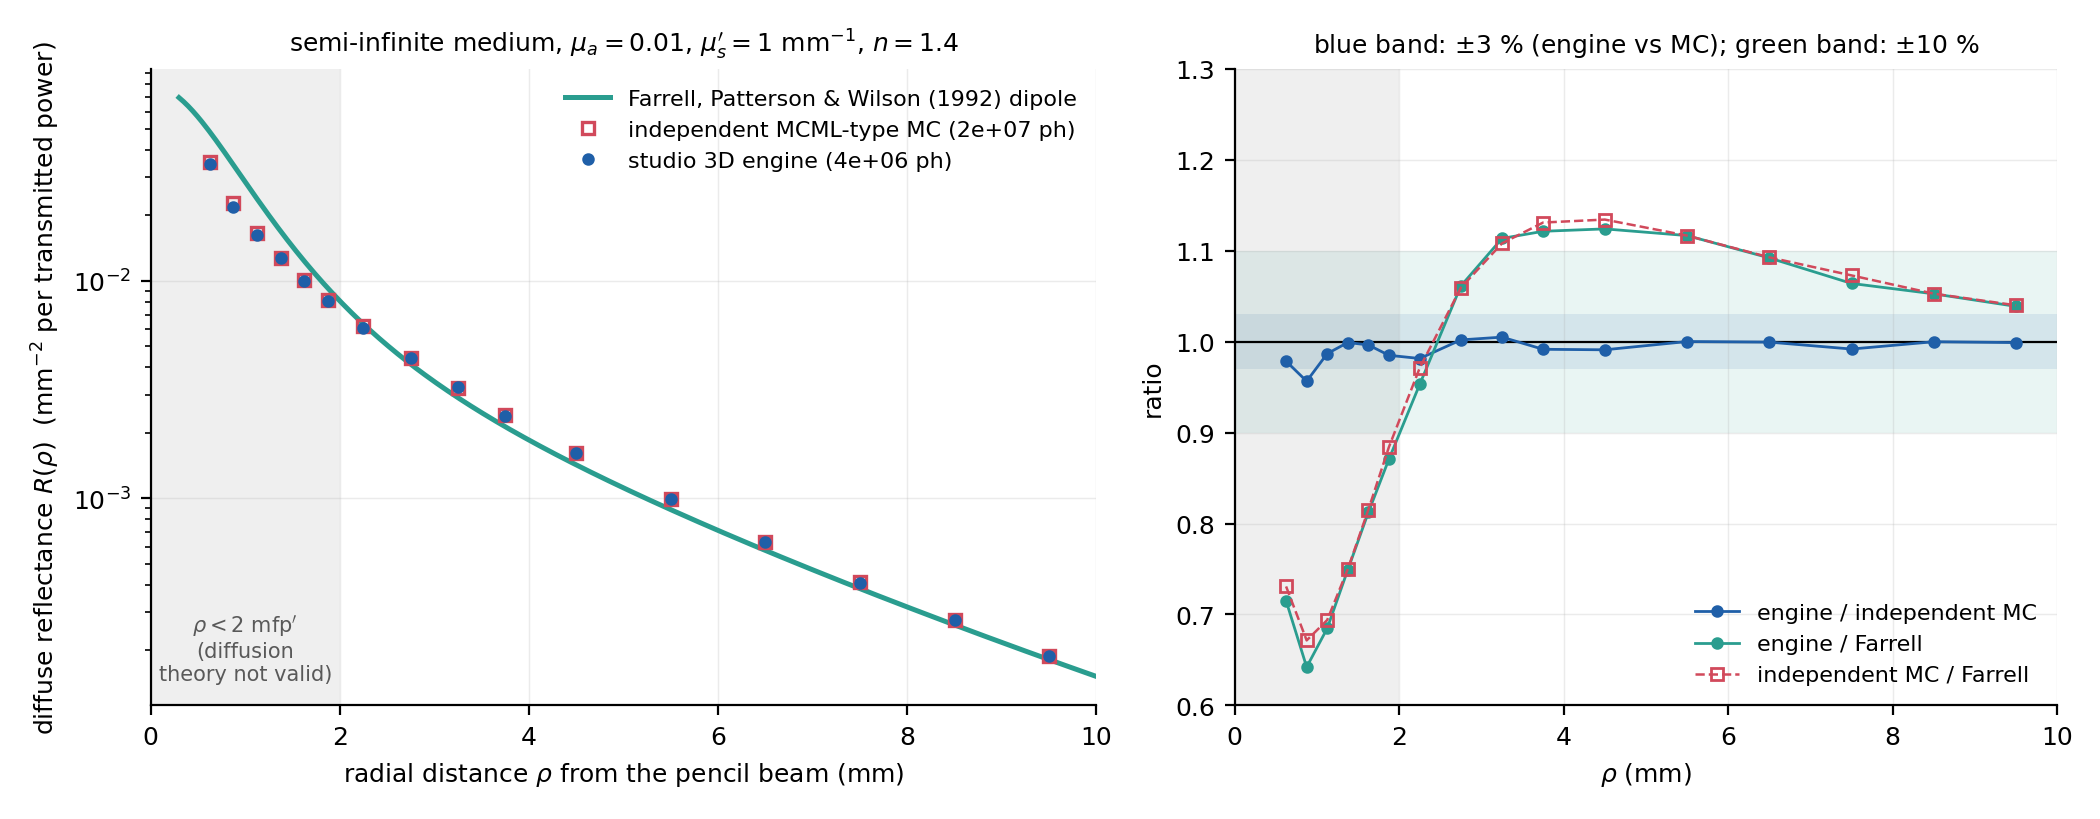
\includegraphics[width=0.92\textwidth]{fig22_radial_reflectance.png}
\caption{Radial diffuse reflectance of a pencil beam on a semi-infinite medium ($\mua=0.01$, $\musp=1$~mm$^{-1}$, $n=1.4$). Left: 3D engine, independent MCML-type Monte Carlo and Farrell--Patterson--Wilson dipole. Right: ratios; the engine follows the independent Monte Carlo within $1.1\,\%$ (blue band $\pm3\,\%$), while the dipole deviates by $-28$ to $-16\,\%$ inside two reduced mean free paths (grey, annulus means) and by up to $+12\,\%$ at 3--6~mm.}
\label{fig:radial}
\end{figure*}
\begin{figure}[!t]
\centering
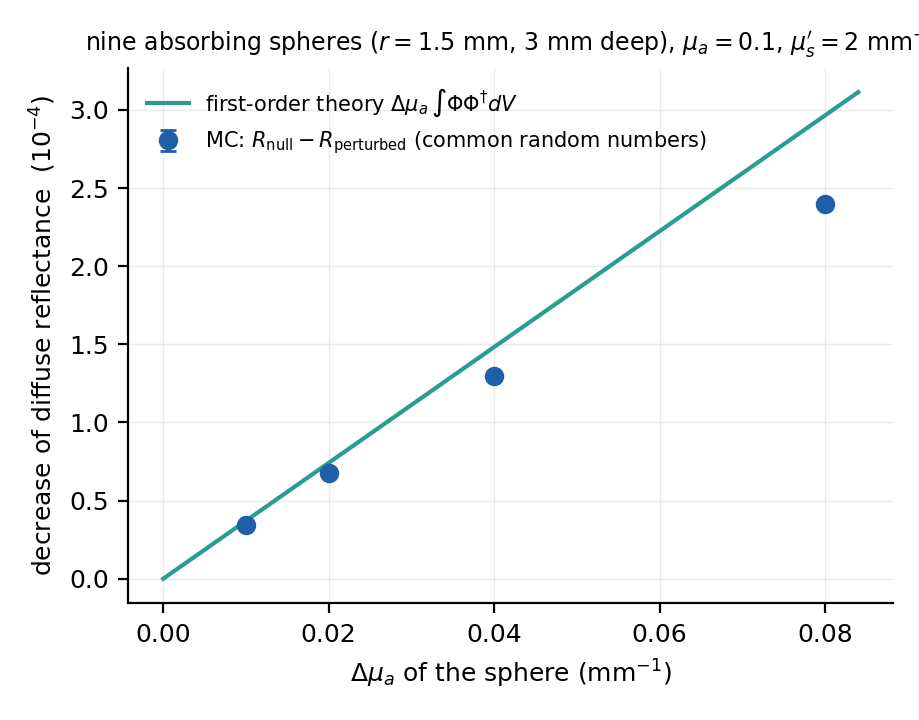
\includegraphics[width=0.85\columnwidth]{fig22b_perturbation.png}
\caption{Perturbation check: decrease of diffuse reflectance caused by absorbing spheres against the increase of their absorption, from the Monte Carlo with common random numbers and from first-order theory.}
\label{fig:perturb}
\end{figure}

\subsection{Sim-to-real: calibrating the twin}
\label{sec:v_s2r}
\emph{Machinery.} The fast forward model of Eq.~\eqref{eq:calib} agrees with a full capture to a maximum relative deviation of $4.1\cdot10^{-4}$ (target 3\,\%). Fitting noisy full captures (eight seeds, global gain, true emission $470/80$~nm, excitation $350/70$~nm) recovers the emission peak with bias $+0.02$~nm (sd $0.06$~nm) at high signal and $+0.31$~nm (sd $0.63$~nm) at low signal, with 95\,\% interval coverage of $100\,\%$ for four of five parameters; without dark subtraction the low-signal peak is biased by $-1.5$~nm.

\emph{Collagen.} For six measured collagen ROIs (Pepsin and Acetic Acid samples) a one-component twin with per-excitation gain and a smooth throughput correction reaches $R^2=0.80$--$0.92$ and a mean spectral angle (SAM) of $6.2$--$7.8^\circ$, against $R^2=0.21$--$0.78$ and $11.0$--$16.9^\circ$ for the nominal instrument (Fig.~\ref{fig:s2r}; Pepsin ROI 2: $R^2=0.919$, SAM $7.0^\circ$ against $0.638$ and $14.9^\circ$). Two components are no better and have a higher BIC. The calibration exposes what is not identifiable: the Nuance window starts at 420~nm, so the emission peak sits on its 380~nm bound; the identifiable descriptors are the centroid above 420~nm (498--505~nm) and the red half-maximum (516--526~nm). The fitted per-excitation gains reveal a radiometric inconsistency of the processed collagen data (a step of about $10^3$ between 340 and 365~nm), which a global-gain model would hide. Refitting under alternative instruments (LCTF FWHM 10/14~nm, long-pass 405/420~nm, UV-enhanced CCD) moves the centroid only within 497--499~nm, but an unphysical flat LCTF throughput moves descriptors by 20--50~nm, so the calibrated emission is conditional on the LCTF curve.

\emph{Hold-out validation} (Fig.~\ref{fig:holdout}; mean SAM). B1, calibrate on three excitations and predict the other three (six ROIs, four splits): corrected twin $8.4^\circ$, twin with ripple $8.6^\circ$, two components $12.3^\circ$, nominal $14.2^\circ$, empirical pooled spectrum $7.7^\circ$, flat $23.7^\circ$ (in-sample refit $6.4^\circ$). B2, calibrate on one ROI and predict another (30 pairs): $7.8^\circ$ (same dataset) and $7.4^\circ$ (other dataset), empirical $6.9^\circ/6.7^\circ$, flat $23.7^\circ$. B3, droplets with global gain, train on 310/340/385/415~nm and predict 325/365/400~nm absolutely without refitting a gain (16 drops): median $R^2=0.956$ (nominal $0.951$), median SAM $6.0^\circ$, median $|\ln(\text{predicted}/\text{measured peak})|=0.17$. The twin therefore predicts held-out excitations, samples and datasets with SAM about $1$--$2^\circ$ above its in-sample value and removes about $90\,\%$ of the flat-baseline error, but it does \emph{not} beat a non-parametric copy of another measured spectrum, and the excitation-dependent shape changes of collagen are not captured by one or two components. Its advantage is that it transfers to instrument settings that an empirical copy cannot represent. Scattering of the measured samples is not identifiable: all bands start at least 25--30~nm above the excitation line and there is no flat-field white reference.

\begin{figure*}[!t]
\centering
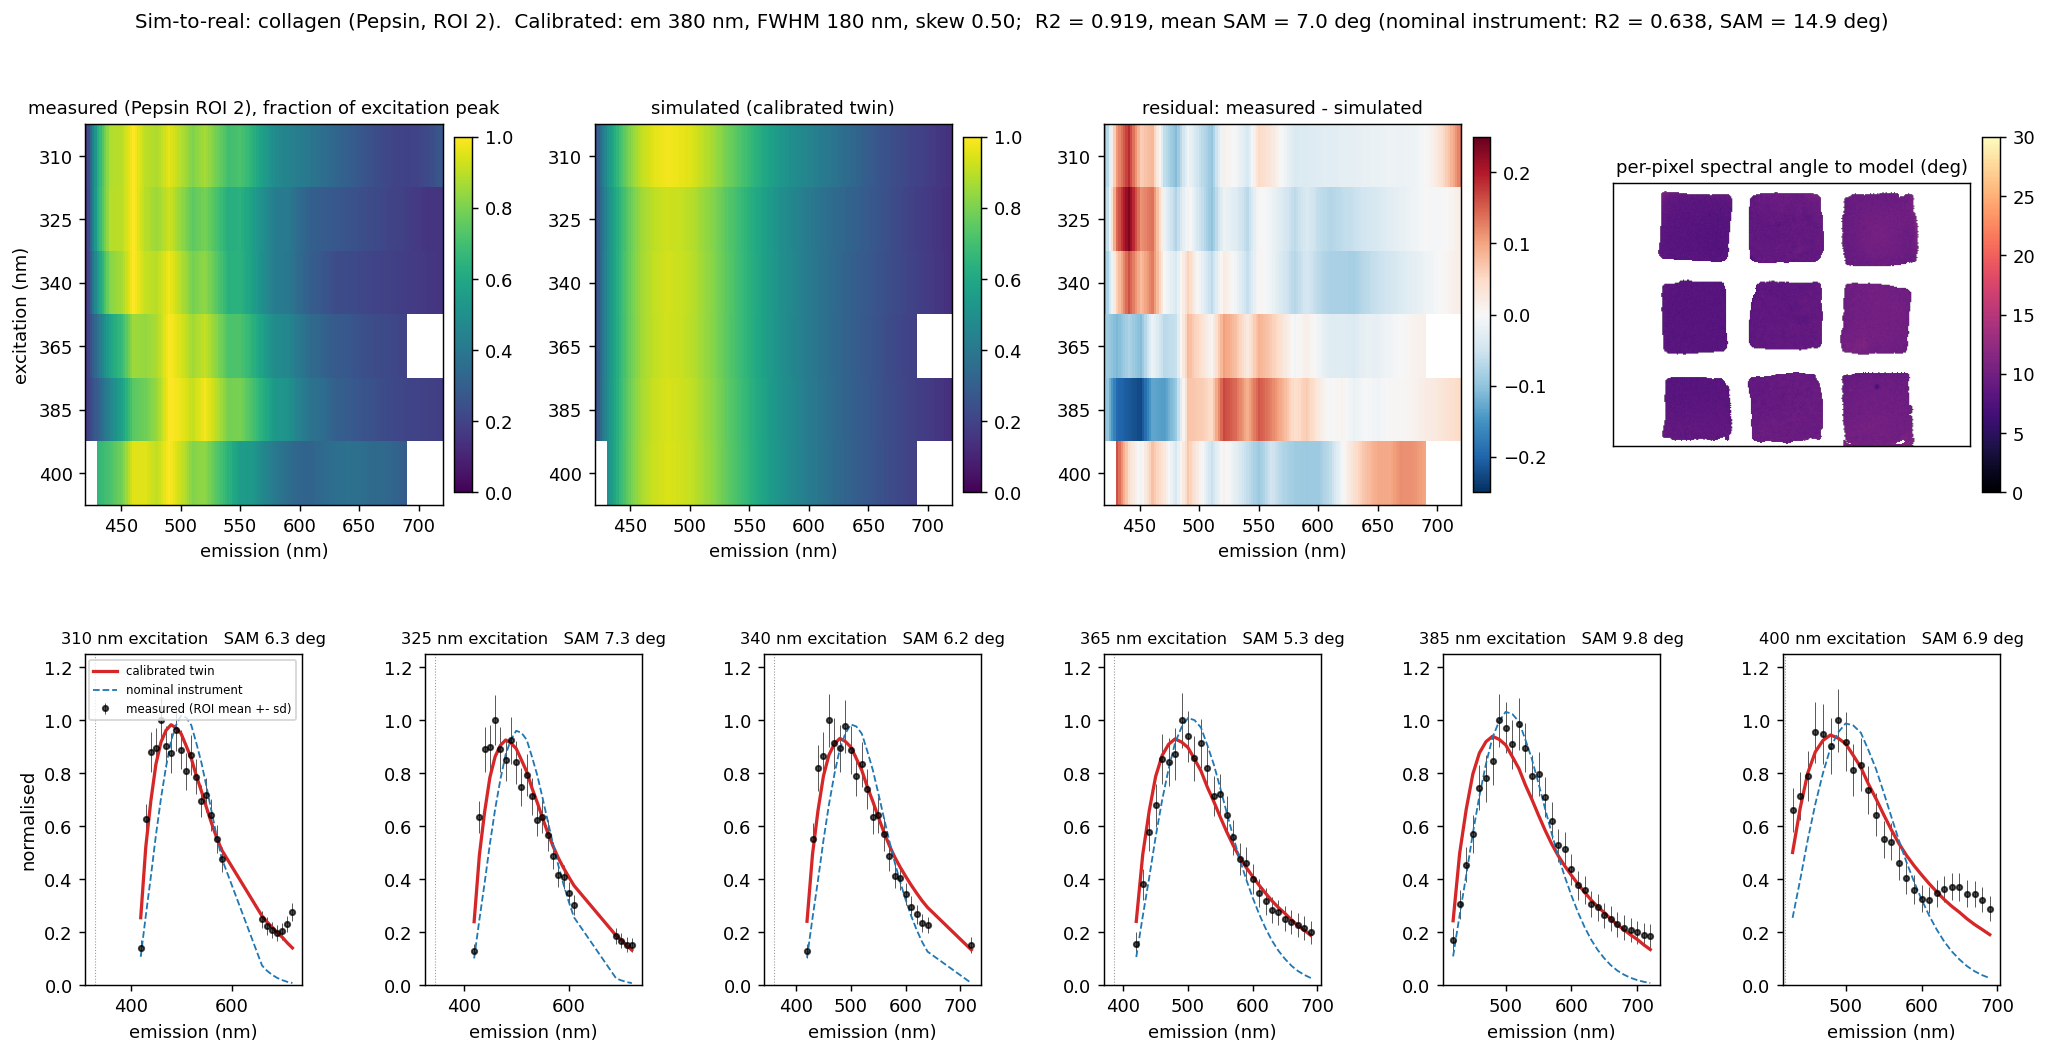
\includegraphics[width=\textwidth]{fig27_sim2real_collagen.png}
\caption{Calibrated twin for collagen (Pepsin ROI 2): measured and simulated EEM, residual, per-pixel spectral angle and spectra at each excitation (calibrated and nominal instrument).}
\label{fig:s2r}
\end{figure*}
\begin{figure*}[!t]
\centering
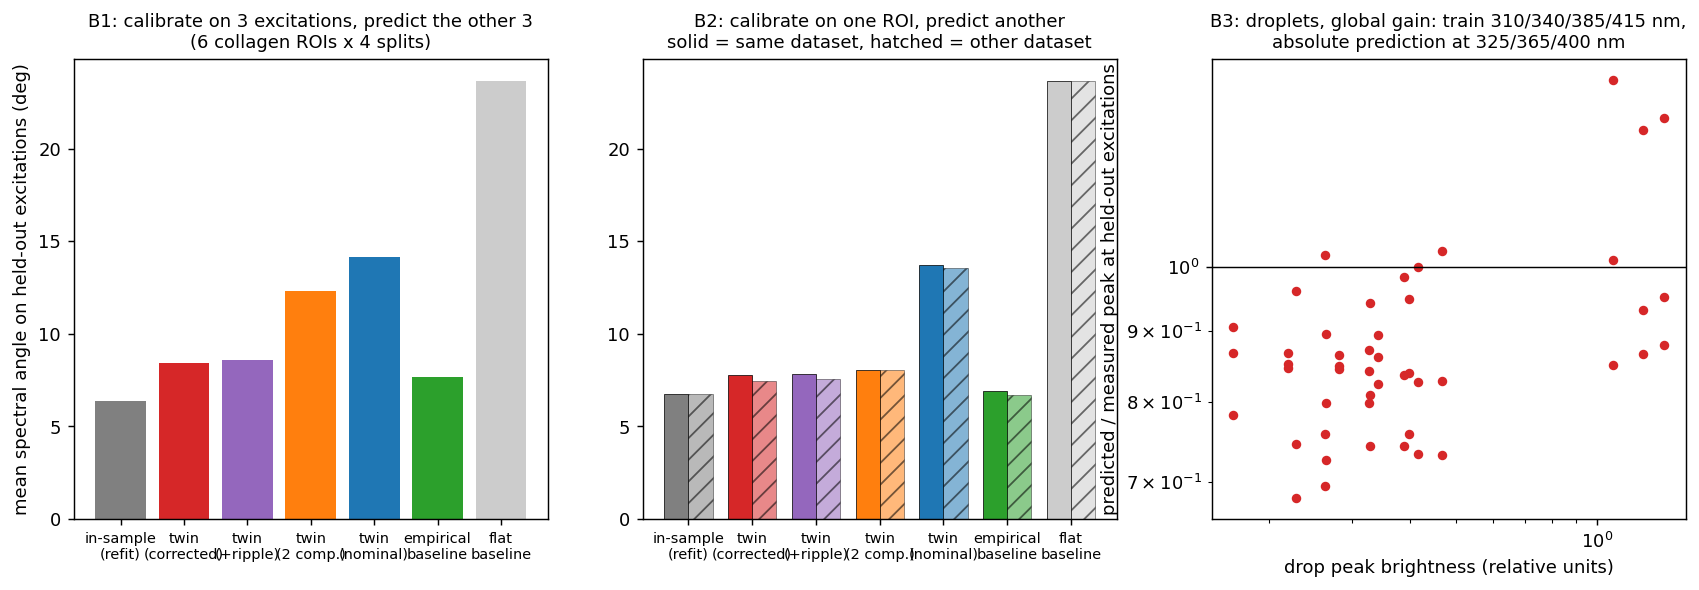
\includegraphics[width=0.92\textwidth]{fig28_sim2real_holdout.png}
\caption{Hold-out validation. B1: held-out excitations. B2: held-out ROIs. B3: absolute amplitude prediction for droplets at held-out lines.}
\label{fig:holdout}
\end{figure*}

\section{Experiments}
\label{sec:experiments}
All experiments use the public API on a tissue-under-collagen scene built from the literature materials of Section~\ref{sec:tissue}: a dense-collagen cover of variable thickness over a papillary-dermis layer carrying NADH, FAD, collagen and elastin, above a reticular-dermis substrate. They ran on an Apple M4 Pro (14 cores) with fixed seeds; each experiment's script, raw runs and provenance record are in the repository. Unless stated, intervals are $95\,\%$ bootstrap intervals. Most studies use the preview or `fast' capture mode, whose per-pixel Monte Carlo noise matters for the pixel-level analyses (Section~\ref{sec:limits}).

\subsection{E2: Cover-thickness response}
\emph{Question.} How fast does the buried signal decay with cover thickness, when does the cover's own autofluorescence take over, and how does the cover distort the emission spectrum?

\emph{Setup.} Collagen thickness $t=0$--$2$~mm (13 values, three seeds), excitation 340, 365, 400 and 430~nm, preview scale $0.25$, $2\cdot10^6$ photons per pass, central $3\times3$ pixels; a blood study with $B=0,1,3\,\%$ at $t=0.1$--$1$~mm (400 and 430~nm); and a gentle (40~mm long) and a steep (8~mm) wedge.

\emph{Results.} The buried-layer signal falls approximately exponentially, by about three decades over 0.5~mm at 340~nm and five decades over 2~mm at 430~nm. The effective depth $\delta_{\rm eff}$ of the fit $I=I_0e^{-t/\delta_{\rm eff}}$ rises from $0.073$ to $0.358$~mm with excitation wavelength (Table~\ref{tab:e2}). Diffusion theory, $\delta=1/\sqrt{3\mua(\mua+\musp)}$ evaluated for the two-way path, agrees at 340 and 365~nm, where absorption is strong ($\mua/\musp\approx0.5$), and overestimates $\delta$ by $1.4$--$1.5\times$ at 400 and 430~nm ($\mua/\musp\approx0.04$--$0.1$), where its assumptions fail; the decay is also not exactly mono-exponential there ($R^2=0.90$--$0.97$), so $\delta_{\rm eff}$ depends on the fit window. The cover's autofluorescence equals that of the buried layer ($50\,\%$ crossover) at $t=0.027$, $0.034$ and $0.045$~mm for 340, 365 and 400~nm, so at UV excitation any cover thicker than about 50~\textmu m is dominated by its own emission; at 430~nm, where collagen barely absorbs, the crossover is at $0.55$~mm (Fig.~\ref{fig:e2a}a). Once the cover dominates, the emission centroid has moved by $-12$ to $-13$~nm (340, 365~nm), $-29$~nm (400~nm) and $-65$~nm (430~nm), i.e.\ to the collagen emission (Fig.~\ref{fig:e2a}b), and the blue/red ratio, which grows by $1.5$--$2.5\times$ already at 25--50~\textmu m, reaches $2\cdot10^2$--$3\cdot10^2$ in the UV as the buried layer's red and green emission is lost first. Blood in the cover at $t=0.25$~mm reduces the buried fluorescence to $0.30$ ($B=1\,\%$) and $0.09$ ($3\,\%$) at 400~nm and to $0.32$ and $0.057$ at 430~nm, within the Soret band; the ratio to the blood-free spectrum shows the HbO$_2$ dips near 542 and 577~nm. The magnitude of the blue/red ratio with blood is uncertain (standard errors up to $100\,\%$ at $t\ge0.5$~mm with three seeds); only its monotone rise with $B$ and $t$ is robust. For the wedges, the ratio of the 3D wedge response to the 1D uniform-block response of the same local thickness has a mean log-ratio of $-0.03\pm0.03$ (400~nm) and $-0.10\pm0.04$ (430~nm) for the gentle wedge and $+0.12\pm0.03$ and $+0.13\pm0.05$ for the steep one, with no trend with thickness. The uniform-block response therefore predicts the wedge to about $10$--$15\,\%$. The lateral blur could not be identified: the fitted width sat at a bound of the search grid in most cases, so this is a null result at two seeds and $2\cdot10^6$ photons, not a measurement.

\begin{table}[!t]
\caption{E2: effective penetration depth of the buried signal (MC fit, $95\,\%$ bootstrap interval) against two-way diffusion theory.}
\label{tab:e2}
\centering\small
\begin{tabular}{@{}cccc@{}}
\toprule
$\lex$ (nm) & $\delta_{\rm eff}$ (mm) & diffusion (mm) & MC$/$diffusion\\
\midrule
340 & $0.073\;[0.057,0.084]$ & $0.068$ & $1.07$\\
365 & $0.105\;[0.070,0.132]$ & $0.096$ & $1.10$\\
400 & $0.199\;[0.164,0.199]$ & $0.300$ & $0.66$\\
430 & $0.358\;[0.219,0.436]$ & $0.496$ & $0.72$\\
\bottomrule
\end{tabular}
\end{table}

\begin{figure*}[!t]
\centering
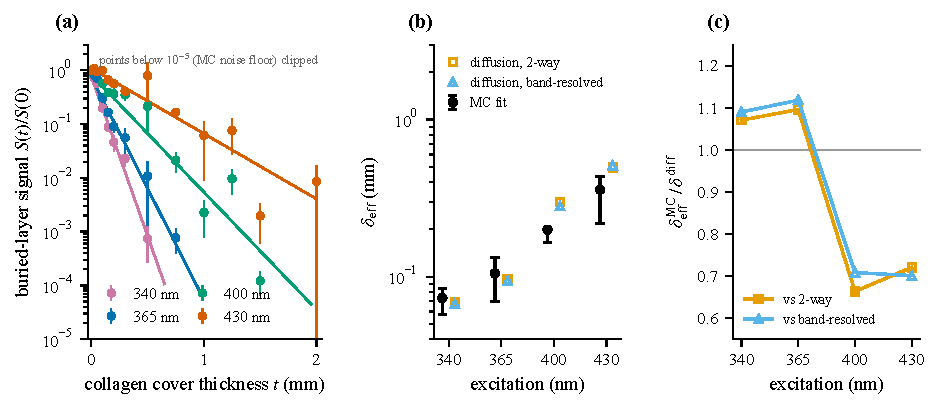
\includegraphics[width=0.7\textwidth]{E2_penetration.pdf}\\[2mm]
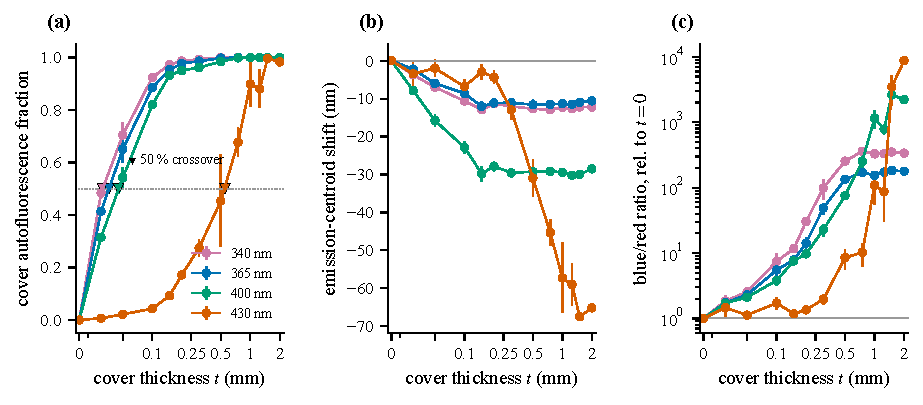
\includegraphics[width=0.7\textwidth]{E2_fraction_distortion.pdf}
\caption{E2, cover-thickness response (three seeds; error bars show the uncertainty over seeds). \emph{Top:} (a) buried-layer signal against collagen thickness with exponential fits (points below $10^{-5}$ of the thin-cover signal, the Monte Carlo floor, are clipped); (b) fitted $\delta_{\rm eff}$ against two-way and band-resolved diffusion theory; (c) their ratio. \emph{Bottom:} (a) fraction of the signal that is cover autofluorescence, with $50\,\%$ crossovers marked; (b) emission-centroid shift relative to $t=0$; (c) blue/red band ratio relative to $t=0$ (log scale).}
\label{fig:e2a}
\end{figure*}

\emph{Take-home.} At 340--365~nm the buried signal is confined to the top $0.1$~mm and the cover's autofluorescence takes over within $50$~\textmu m, while at 430~nm the cover is nearly transparent to the excitation but absorbs the Soret band if it contains blood.

\subsection{E3: Global sensitivity and confounders}
\emph{Question.} How much of the variance of the optical redox ratio $\mathrm{FAD}/(\mathrm{FAD}+\mathrm{NADH})$ is caused by the cover, as opposed to the metabolic state, and does ratioing against an elastic or cover-autofluorescence channel remove it?

\emph{Setup.} Eight inputs: cover thickness ($0.1$--$1$~mm), $\musp(500)$ ($1.5$--$4.5$~mm$^{-1}$) and $b_{\rm Mie}$ ($0.5$--$1.5$) of the cover, blood fraction ($0.2$--$5\,\%$), StO$_2$ ($0.4$--$1$), buried NADH ($20$--$150$~\textmu M) and FAD ($10$--$100$~\textmu M) and collagen concentration ($300$--$1500$~\textmu M). Saltelli design with $N=64$ base rows (640 runs, none failed; mean capture 2.7~s, $10^6$ photons per pass), 1000 bootstrap resamples, Morris with eight trajectories (72 runs) and a noise study of six points with four replicates. Outputs: the NADH band (365~nm excitation, 440--480~nm), the FAD band (450~nm, 510--550~nm), the redox ratio, and the peak wavelength. $N=64$ is below the $N\ge256$ we planned, which limits the tightness of the intervals; the Sobol' indices below use the centred estimator of Section~\ref{sec:toolkit}.

\emph{Results.} The Monte Carlo noise floor is $0.007$ for the redox ratio, $0.011$ for the NADH and FAD bands, and $0.447$ for the peak wavelength, which is therefore inconclusive. For the redox ratio, cover thickness alone has $S_i=0.49$ $[0.23,0.81]$ and $S_{T_i}=1.04$ $[0.68,1.57]$, FAD concentration $S_i=0.22$ $[0.09,0.37]$, and NADH concentration $S_i=-0.06$ $[-0.18,0.06]$, indistinguishable from zero; the other inputs have $S_i\le0.10$. Summed over groups, the cover inputs (thickness, $\musp$, $b_{\rm Mie}$, blood, StO$_2$, collagen fluorescence) carry a first-order share of $0.66$ against $0.16$ for NADH and FAD (Table~\ref{tab:e3}, Fig.~\ref{fig:e3}), and a Gaussian-process surrogate (cross-validated $R^2=0.73$) gives group total indices of $0.91$ and $0.16$. The sum of first-order indices of the redox ratio is $0.82$; for the NADH and FAD bands the cover share is $0.73$ and $0.87$. Morris screening agrees (rank correlation of $\mu^*$ with $S_{T}$ of $0.83$; thickness, then FAD, then $\musp$ by $\mu^*$), as does the scatter (Spearman $\rho=-0.67$ against thickness, $+0.04$ against NADH). Ratioing against an elastic channel (FAD$/$elastic), a cover-autofluorescence channel (NADH$/$AF) or both does not reduce the cover share: the group total index stays at $0.93$--$0.95$ against $0.91$ without correction.

\emph{Reliability.} Single-input total indices are noisy at $N=64$ and some exceed one (thickness for the redox ratio, $1.04$; blood for the NADH band, $1.13$), so we use $S_{T_i}$ only as ranks with intervals. The NADH$/$AF ratio has $\sum_iS_i=1.85$ and is unreliable for absolute shares. The bootstrap intervals of the group indices are degenerate (lower bound of the metabolic $S_T$ interval, $0.17$, above its estimate of $0.16$), so only the point estimates are usable. An earlier analysis with an uncentred first-order estimator gave a redox-ratio $\sum_iS_i=-0.04$ and peak-wavelength $\sum_iS_i=-13$; the numbers here come from re-analysing the stored runs with the centred estimator (ST and Morris were unaffected).

\begin{table}[!t]
\caption{E3: grouped Sobol' indices of the cover inputs and of the metabolic inputs (NADH, FAD), $N=64$. $S_1$ from the centred Saltelli estimator, $S_T$ from Jansen; $S_T$ values are noisy (see text).}
\label{tab:e3}
\centering\footnotesize\setlength{\tabcolsep}{3pt}
\begin{tabular}{@{}lcccc@{}}
\toprule
output & cover $S_1$ & metab.\ $S_1$ & cover $S_T$ & metab.\ $S_T$\\
\midrule
NADH band & $0.73$ & $-0.03$ & $1.40$ & $0.04$\\
FAD band & $0.87$ & $0.22$ & $2.09$ & $0.52$\\
redox ratio & $0.66$ & $0.16$ & $2.21$ & $0.40$\\
peak wavelength$^{*}$ & $0.31$ & $0.21$ & $3.51$ & $1.23$\\
\bottomrule
\end{tabular}\\[1mm]
{\footnotesize $^{*}$Noise floor $0.447$; inconclusive.}
\end{table}

\begin{figure*}[!t]
\centering
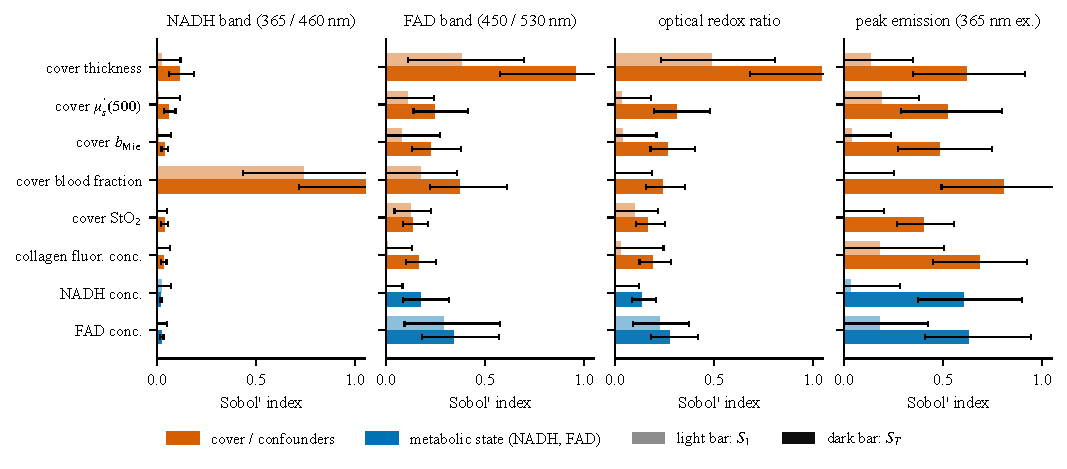
\includegraphics[width=0.7\textwidth]{E3_sobol.pdf}
\caption{E3, Sobol' indices of eight inputs for four outputs ($N=64$ base rows, $95\,\%$ bootstrap intervals). Light bars: first-order $S_i$; dark bars: total $S_{T_i}$; orange: cover and confounders, blue: metabolic state. Thickness and blood dominate the NADH and FAD bands and the redox ratio.}
\label{fig:e3}
\end{figure*}

\emph{Take-home.} In this model, the redox ratio is mainly a measure of the cover (thickness alone $S_i=0.49$), and the simple ratio corrections tested do not remove this.

\subsection{E4: Inclusion detectability}
\todo{E4 results pending}

\subsection{E5: Information-optimal acquisition}
\emph{Question.} Which channels of the $8\times31=248$-channel lab-replica protocol carry the information on cover thickness, how many reach the Cram\'er--Rao bound (CRLB) of the full protocol, and how robust is this to model error?

\emph{Setup.} Thickness surrogate on eight grid points over $0.05$--$1.5$~mm (leave-one-out relative RMS $6.4\,\%$, maximum $9.2\,\%$), scale $0.25$, ROI of 3744 full-resolution pixels, full-protocol exposure 233~s. The model-error level $\epsilon$ of Eq.~\eqref{eq:modelerr} is $0$, $0.5$, $1$, $2$, $5$ and $7\,\%$ (the last is the $7.0\,\%$ derived from the sim-to-real fits). Greedy and exchange-refined D-optimal selection are compared with 40 random subsets (median, IQR), uniform subsets, and the label-free selection of our earlier work~\cite{meloyan2025scirep} ($k=8$, two seeds). Efficiency is the ratio of the standard deviation of 200 ML fits to the CRLB.

\emph{Results.} At $t=0.6$~mm the photon-limited CRLB for thickness is $0.26$~\textmu m alone, $0.90$~\textmu m with an unknown amplitude and $1.05$~\textmu m with per-excitation gains. Model error lifts this floor roughly linearly in $\epsilon$ (about $1.3$~\textmu m per percent), to $2.2$--$9.5$~\textmu m for $\epsilon=0.5$--$7\,\%$ (Table~\ref{tab:e5}, Fig.~\ref{fig:e5a}): already at $0.5\,\%$ the floor is $2.4\times$ the photon-limited one, so precision is systematics-limited. The photon-limited values are bounds on information and not achievable precisions; the floors are still one to two orders of magnitude below the $25$--$200$~\textmu m errors of E6, which the variance-only CRLB cannot contain. For thickness and amplitude, 28 channels come within $10\,\%$ of the full-protocol CRLB at $\epsilon=0$ ($81\,\%$ less exposure time) and $28$--$45$ channels for $\epsilon>0$ ($88$--$94\,\%$ less), i.e.\ about $12\,\%$ of 248; for the joint (thickness, NADH, $\musp$) problem 13 channels suffice photon-limited and 20--27 under model error. Random and uniform subsets reach this level only with $k\ge200$. At $k=8$ the information-optimal set gives a CRLB $1.24$~\textmu m against a random median of $12.6$~\textmu m ($10\times$) at $\epsilon=0$, and $6.7$ against $34$~\textmu m ($5\times$) at $\epsilon=2\,\%$. The optimal set depends on $\epsilon$ (Fig.~\ref{fig:e5a}a): photon-limited selection picks UV-excited blue channels (310--325~nm excitation, 420--480~nm emission), which have high absolute signal, while for $\epsilon\ge0.5\,\%$ it moves to 415--430~nm excitation and 455--570~nm emission with larger relative thickness sensitivity (Jaccard index with the photon-limited set $0.14$ at $0.5\,\%$ and $0.07$ for $\epsilon\ge2\,\%$). Using the photon-optimal set when $\epsilon=2\,\%$ costs $28$~\textmu m instead of $6.7$~\textmu m. The label-free selection is $2$--$2.5$~\textmu m photon-limited ($2\times$ worse than optimal, $5\times$ better than random) but $39$--$44$~\textmu m at $\epsilon=2\,\%$, comparable to random ($34$~\textmu m). The photon-only efficiency of the ML fit is $1.01$ and $0.99$ at $t=0.25$ and $0.6$~mm ($0.95$--$1.03$ for $k=8$); at $1.1$~mm the surrogate bias ($-230$~\textmu m) invalidates the comparison. With $\epsilon=2\,\%$ the ratio is $1.13$ to $1.64$ for all channels and $0.99$ to $4.2$ for $k=8$, larger where bias exceeds the standard deviation.

\emph{Caveats.} The finite-difference and surrogate Jacobians disagree at $t=0.9$~mm (standard deviations $0.39$ and $0.92$~\textmu m, Monte Carlo noise in the differences); the exposure allocation of the design tool did not beat equal allocation in this scene and is not used; and this is one scene and one ROI.

\begin{table}[!t]
\caption{E5: thickness precision floor at $t=0.6$~mm (thickness and amplitude unknown) and number $k$ of greedy-selected channels within $10\,\%$ of the full-protocol bound, against model error $\epsilon$.}
\label{tab:e5}
\centering\small
\begin{tabular}{@{}lcccccc@{}}
\toprule
$\epsilon$ (\%) & 0 & 0.5 & 1 & 2 & 5 & 7\\
\midrule
floor (\textmu m) & $0.90$ & $2.2$ & $2.8$ & $4.0$ & $7.3$ & $9.5$\\
$k$ (of 248) & 28 & 35 & 28 & 30 & 40 & 45\\
\bottomrule
\end{tabular}
\end{table}

\begin{figure*}[!t]
\centering
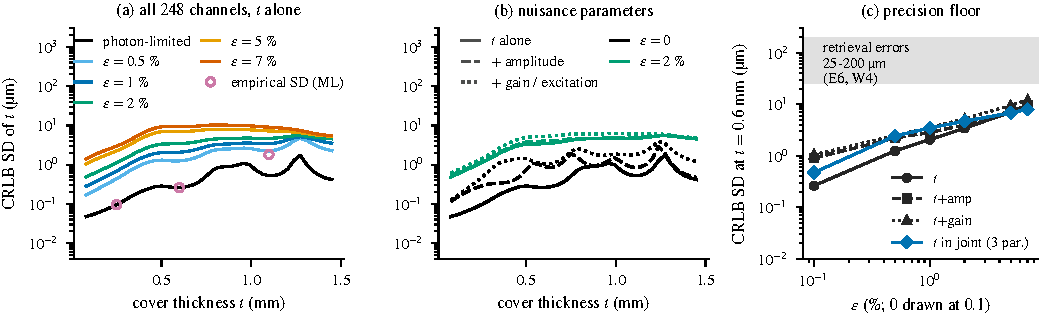
\includegraphics[width=0.72\textwidth]{E5_precision.pdf}\\[2mm]
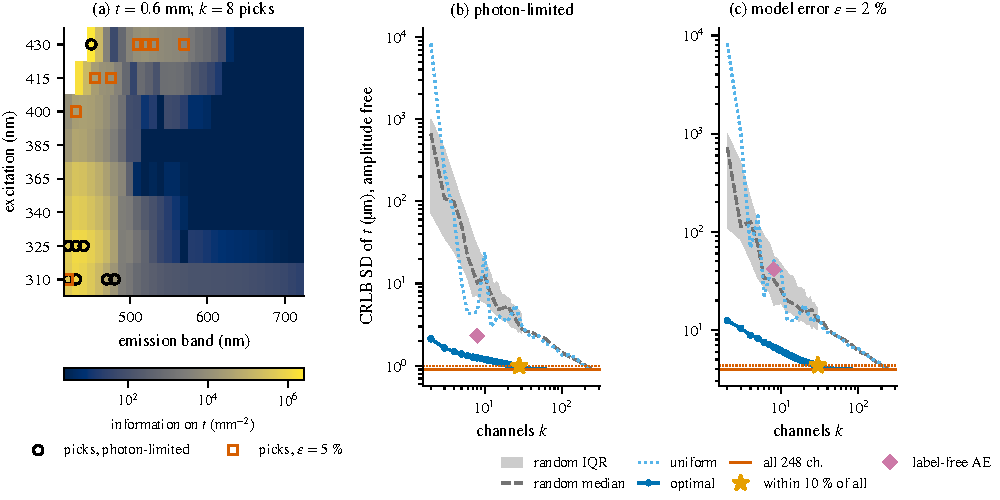
\includegraphics[width=0.6\textwidth]{E5_design.pdf}
\caption{E5. \emph{Top:} CRLB standard deviation of the cover thickness, (a) for all 248 channels against thickness and model error $\epsilon=0$ to $7\,\%$, (b) with nuisance parameters (amplitude, per-excitation gain, joint fit with NADH and $\musp$), (c) at $t=0.6$~mm against $\epsilon$; the grey band marks the retrieval errors of E6. \emph{Bottom:} (a) information on thickness per channel at $t=0.6$~mm with the eight channels selected at $\epsilon=0$ (circles) and $5\,\%$ (squares); (b, c) CRLB against the number of channels $k$ for information-optimal, random (median, IQR) and uniform selection and the label-free autoencoder selection, at $\epsilon=0$ and $2\,\%$ (stars mark the $k$ within $10\,\%$ of the full-protocol bound).}
\label{fig:e5a}
\end{figure*}

\emph{Take-home.} About 30 of 248 channels carry the information of the full protocol, but the choice depends on the assumed model error, and photon-limited CRLBs overstate what can be retrieved.

\subsection{E6: Thickness mapping}
\emph{Question.} How accurately can the cover thickness be mapped on a wedge, and are the retrieval intervals calibrated?

\emph{Setup.} Tile retrieval ($4\times4$ output pixels, scale $0.25$) with the surrogate fit of Section~\ref{sec:toolkit} on a tissue wedge ($0.1$--$1.4$~mm, 144 tiles, 248 channels) and a phantom wedge (2--0~mm, 108 tiles, six excitations), with free amplitude, three exposure levels ($0.003$, $0.03$ and $1$ of nominal), photon-only or $\epsilon=2\,\%$ weights and standard errors, bootstrap intervals over tiles, and channel sets ``all'', $k=8$ information-optimal and five random $k=8$ draws. The surrogate is trained on uniform-thickness blocks, so lateral transport at the wedge slope is unmodelled. One noise realisation.

\emph{Results.} At nominal exposure the tissue wedge is retrieved with an RMSE of $405$~\textmu m ($343$--$469$) using photon-only weights and $262$~\textmu m ($220$--$316$) with $\epsilon=2\,\%$ (bias $+89$ and $+25$~\textmu m); the phantom reaches $184$ and $160$~\textmu m. The phantom RMSE rises only from $184$ to $246$~\textmu m (photon-only) when exposure falls from 1 to $0.003$, while the tissue RMSE reaches $776$~\textmu m at $0.003$ (Fig.~\ref{fig:e6}), so at nominal exposure accuracy is limited by model bias, not photons. The photon-limited tile CRLB is $17$~\textmu m (tissue) and $2.7$~\textmu m (phantom) at nominal exposure, so the observed RMSE exceeds it by $15$--$70\times$. Nominal $95\,\%$ coverage is $8\,\%$ (tissue) and $5\,\%$ (phantom) with photon-only standard errors (mean $23$ and $3$~\textmu m against errors of $100$--$400$~\textmu m), and $19$ and $13\,\%$ with $\epsilon=2\,\%$; coverage looks acceptable at the lowest exposure (0.88 for the phantom) only because the photon standard error is large. Eight information-optimal channels give $274$~\textmu m on the tissue (coverage $0.54$) against $405$ (photon-only) and $262$~\textmu m (all channels), and $498\pm91$~\textmu m for random $k=8$ sets; on the phantom, however, all channels ($160$--$184$~\textmu m) beat the optimal $k=8$ set ($247$--$335$~\textmu m), which was optimised on the tissue Fisher information for thickness, not on mapping accuracy, so CRLB-optimality does not guarantee low bias. In the tissue the RMSE is nearly flat with thickness ($260$, $261$ and $266$~\textmu m in bins $0$--$0.5$, $0.5$--$1$ and $1$--$2.1$~mm).

\begin{figure*}[!t]
\centering
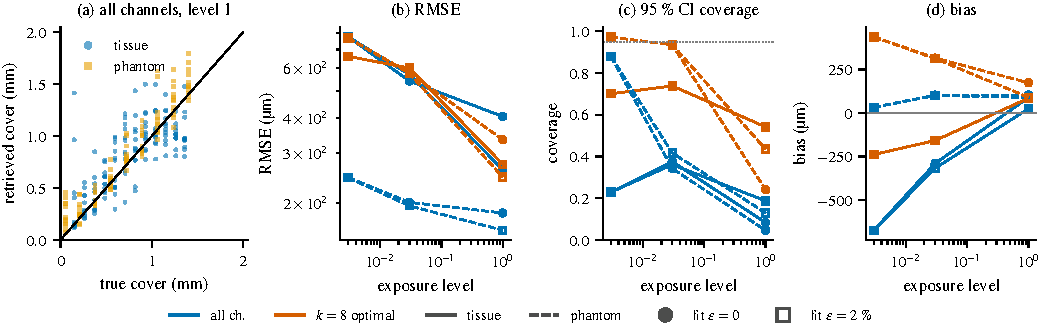
\includegraphics[width=0.75\textwidth]{E6_thickness_mapping.pdf}
\caption{E6, thickness mapping on a tissue wedge and a phantom wedge. (a) Retrieved against true thickness at nominal exposure (all channels); (b) RMSE, (c) nominal $95\,\%$ interval coverage and (d) bias against relative exposure for all channels and eight information-optimal channels, with photon-only ($\epsilon=0$) or $\epsilon=2\,\%$ weights. Accuracy saturates at about 160--260~\textmu m while the photon-only intervals cover only $5$--$8\,\%$ of the tiles.}
\label{fig:e6}
\end{figure*}

\emph{Take-home.} Wedge thickness is retrievable to about $160$--$260$~\textmu m RMSE, limited by model bias; photon-based intervals are over-confident by an order of magnitude, and model-error weighting improves the RMSE by about $35\,\%$ and the coverage $2.5\times$ without restoring nominal coverage.

\subsection{E7: Depth-dependent unmixing failure}
\emph{Question.} How does cover depth bias the linear unmixing of buried NADH, FAD and the matrix, and does a depth-matched library remove the bias?

\emph{Setup.} Uniform cover $t=0.05$--$1.3$~mm (eight values), noisy `fast' capture (scale $0.25$), NNLS on the mean spectrum of 24 random ROI pixels, groups NADH, FAD, matrix (collagen and elastin) and scatter (elastic, glint, leakage), joint 8-line EEM (also 4-line and 365~nm only). Signatures and ground truth are taken from the \emph{Explain pixel} decomposition of the \emph{same} 24 pixels (oracle libraries); a held-out variant builds signatures from 12 pixels and tests on the other 12. Errors are normalised by the true signal at $0.05$~mm. A first version took endmembers from three pixels and ground truth from other pixels, and the per-pixel Monte Carlo noise of the `fast' capture (about $39\,\%$ per channel, median over channels) then produced errors of $-33$ to $+60\,\%$ at $0.05$~mm; this was an artefact and is removed here (noisy floor at $0.05$~mm: NADH $+1\,\%$, FAD $+6\,\%$; noise-free: exactly zero).

\emph{Results.} The detected NADH signal falls $10^4$-fold between $0.05$ and $1.3$~mm ($53\,\%$ left at $0.1$, $2.2\,\%$ at $0.4$, $0.34\,\%$ at $0.6$~mm), FAD $50$-fold, while matrix and scatter rise by $1.5$--$1.8\times$. A library measured on thinly covered material assigns NADH $=0$ for every $t\ge0.1$~mm although the true NADH is $53\,\%$ of its shallow value at $0.1$~mm (noise-free data give the same, so it is bias), which makes the redox-ratio error $+0.59$ at $0.1$~mm (Table~\ref{tab:e7}, Fig.~\ref{fig:e7}). With endmembers simulated at the right depth, NADH and FAD are recovered to within $\pm6\,\%$ of the shallow signal up to $0.6$~mm (redox error $\le0.05$ for $0.2$--$0.6$~mm; the $+0.54$ at $0.1$~mm is a noise-limited outlier of the joint-8 fit). Beyond about $0.6$~mm failure is a detection limit, not a bias: the NADH estimate sits at a noise floor of $1$--$2.5\,\%$ of the shallow signal while the true value is $\le0.3\,\%$, so the redox ratio saturates wrongly ($-0.73$ at $1.3$~mm), and per-layer endmembers (condition number $5$--$34$) do not help. In the held-out variant, signature noise alone gives redox errors of $-0.4$ to $-0.5$ at $0.4$--$0.6$~mm and $-1.0$ at $1.3$~mm, which is partly an artefact of the `fast' noise. The 4-line set behaves like the 8-line set (condition number $6$--$11$ against $4$--$7$); 365~nm alone is ill-conditioned (condition number $107$ at $0.05$~mm, $8\cdot10^3$ at $0.6$~mm).

\begin{table}[!t]
\caption{E7: error of the unmixed redox ratio FAD$/$(FAD$+$NADH) (estimated minus true; true value $0.30$ at $0.05$~mm, $0.88$ at $0.4$~mm, $1.00$ for $\ge1$~mm), joint 8-line EEM, noisy data.}
\label{tab:e7}
\centering\footnotesize\setlength{\tabcolsep}{3pt}
\begin{tabular}{@{}lccccc@{}}
\toprule
library, $t$ (mm) & 0.05 & 0.1 & 0.4 & 0.6 & 1.3\\
\midrule
thin-cover & $+0.009$ & $+0.59$ & $+0.119$ & $+0.017$ & $0.000$\\
depth-matched & $+0.009$ & $+0.54$ & $-0.031$ & $+0.017$ & $-0.726$\\
depth, per layer & $+0.011$ & $+0.04$ & $+0.077$ & $-0.010$ & $-0.702$\\
depth, held-out & $-0.003$ & $+0.37$ & $-0.467$ & $-0.398$ & $-1.000$\\
\bottomrule
\end{tabular}
\end{table}

\begin{figure*}[!t]
\centering
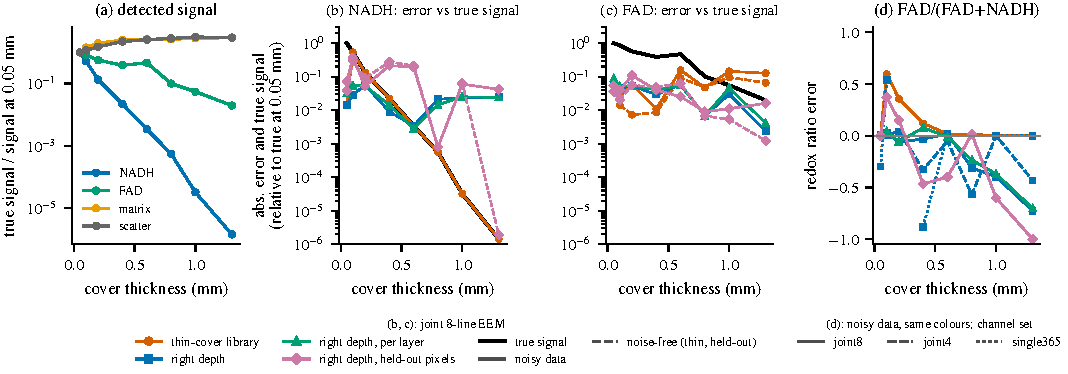
\includegraphics[width=0.85\textwidth]{E7_depth_unmixing.pdf}
\caption{E7, unmixing against cover thickness. (a) Detected signal of each group relative to $0.05$~mm; (b, c) absolute error of NADH and FAD abundance relative to the shallow true signal for the four libraries (the black line is the true signal); (d) redox-ratio error for joint 8-line, 4-line and 365~nm-only channel sets. The thin-cover library fails from $0.1$~mm; depth-matched endmembers help until the NADH signal falls below the noise floor.}
\label{fig:e7}
\end{figure*}

\emph{Take-home.} Unmixing with a thin-cover library fails by spectral distortion between $0.1$ and $0.6$~mm, where a depth-matched library repairs it to a few percent; beyond that, NADH is below the noise floor and no library recovers it.

\subsection{E8: Sim-to-real consolidation}
\emph{Question.} How well does the calibrated twin predict measured spectra, and does the calibrated collagen emission keep its shape when it is transported through the 3D scene?

\emph{Setup.} Table~\ref{tab:e8} consolidates the hold-out results of Section~\ref{sec:v_s2r} (mean $\pm$ s.d.\ of the spectral angle in degrees over ROIs and splits; B1 six ROIs with held-out excitations, B2 30 ROI pairs; the droplet test B3 has 16 drops). In addition, the calibrated collagen emission replaces the library collagen in the 3D Monte Carlo for a 3~mm collagen slab and a $0.5$~mm collagen cover on dermis (lab source and Nuance twin, $10^6$ photons, central $40\,\%\times40\,\%$ ROI, bands at least 20~nm above the excitation, 1200~\textmu M), and the simulated emission shape is compared with the measured Pepsin ROI~2 spectrum at each excitation. The measured samples are thin, so this tests whether the calibrated shape survives transport, not whether the simulation predicts a measured thick cover.

\emph{Results.} The one-component twin with throughput correction has $8.4^\circ\pm1.7^\circ$ on held-out excitations (nominal $14.2^\circ$, empirical copy $7.7^\circ$, flat $23.7^\circ$), $7.8^\circ$ and $7.4^\circ$ on held-out ROIs of the same and the other dataset, and a droplet median $R^2=0.956$ at held-out lines without refitting a gain (Table~\ref{tab:e8}); it does not beat an empirical copy. In the cover scenes, the library collagen emission has a mean spectral angle of $52.1^\circ$ (slab) and $51.6^\circ$ (cover on dermis) from the measurement and the calibrated emission $17.2^\circ$ in both scenes; once the ROI-fitted instrument throughput polynomial, a property of the real instrument that the nominal twin lacks, is applied, the angles are $57.4^\circ$ and $58.2^\circ$ (library) and $9.4^\circ$ and $8.6^\circ$ (calibrated; Fig.~\ref{fig:e8}), against $7.0^\circ$ for the thin-layer fit itself. The calibrated shape therefore survives transport with about $1.6^\circ$--$2.4^\circ$ of added deviation after throughput correction. One ROI, one calibration, single seed.

\begin{table}[!t]
\caption{E8: mean spectral angle ($^\circ$, mean $\pm$ s.d.) for held-out excitations (B1) and held-out ROIs of the same (B2 same) and another (B2 other) dataset.}
\label{tab:e8}
\centering\footnotesize\setlength{\tabcolsep}{3pt}
\begin{tabular}{@{}lccc@{}}
\toprule
Model & B1 & B2 same & B2 other \\
\midrule
In-sample refit & 6.4 & -- & -- \\
Twin, corrected (1 c.) & 8.4\,$\pm$\,1.7 & 7.8\,$\pm$\,1.4 & 7.4\,$\pm$\,1.0 \\
Twin + ripple & 8.6\,$\pm$\,1.8 & 7.8\,$\pm$\,1.4 & 7.6\,$\pm$\,1.1 \\
Twin, 2 comp. & 12.3\,$\pm$\,9.3 & 8.0\,$\pm$\,1.4 & 8.1\,$\pm$\,1.2 \\
Twin, nominal & 14.2\,$\pm$\,2.5 & 13.7\,$\pm$\,2.2 & 13.6\,$\pm$\,2.1 \\
Empirical copy & 7.7\,$\pm$\,2.0 & 6.9\,$\pm$\,1.5 & 6.7\,$\pm$\,1.3 \\
Flat spectrum & 23.7\,$\pm$\,2.1 & -- & -- \\
\bottomrule
\end{tabular}
\end{table}

\begin{figure}[!t]
\centering
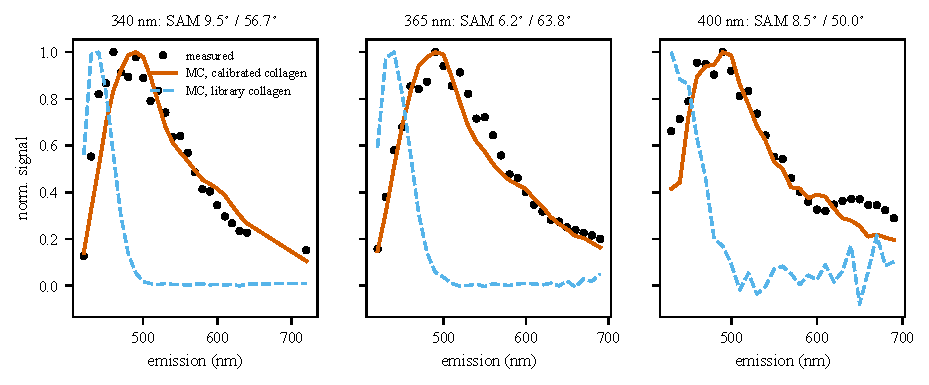
\includegraphics[width=\columnwidth]{E8_cover_check.pdf}
\caption{E8, calibrated collagen emission in the simulated 3~mm collagen slab (normalised): measured spectrum (dots), simulation with the calibrated emission (solid) and with the library collagen (dashed), at three excitations; the titles give the spectral angles (calibrated / library) with the fitted instrument throughput applied.}
\label{fig:e8}
\end{figure}

\emph{Take-home.} With the instrument throughput applied, calibration moves the simulated collagen from about $57^\circ$ to about $9^\circ$ of the measured shape, close to the thin-layer fit ($7^\circ$), but the empirical-copy baseline is not beaten.

\subsection{E9: Label-free segmentation under a cover}
\emph{Question.} How does burial under a collagen cover limit unsupervised separation of tissue types, and does the information-optimal channel selection of E5 help?

\emph{Setup.} 14 captures (Latin-hypercube design, seed 9) of three side-by-side tissue types (NADH-rich, FAD-rich and stroma buried layers, 1~mm) under a dense-collagen wedge ($t_0\in[0,0.3]\to t_1\in[1.0,1.5]$~mm), seven excitations (310--430~nm) by 31 bands $=217$ channels, `fast' mode, $87\times64$ pixels, $3\cdot10^5$ photons per step, about 1900 tissue pixels per capture, $K=3$. Methods: $k$-means and Gaussian mixture on z-scored PCA features (10 components, raw or $3\times3$ spatially binned) and $k$-means on the latent of the convolutional autoencoder of our repository (30 epochs, default sparsity weight, no tuning). Adjusted Rand index (ARI) and NMI against tissue type, as mean $\pm$ s.e.\ over the 14 captures, per bin of local cover thickness; fits are made separately in each bin to remove the thickness gradient. A supervised shrinkage-LDA (four-fold cross-validated accuracy) is shown as a non-label-free reference. A noise check on one scene with two seeds gives a relative pixel noise of $8.2\,\%$ at the dataset photon budget and $7.3\,\%$ at four times the photons, so the Monte Carlo share is about $4.3\,\%$ and the sensor share about $7.0\,\%$ in this (channel-mean-normalised) metric.

\emph{Results.} With $3\times3$ binning, the per-bin ARI of $k$-means falls monotonically with burial (Table~\ref{tab:e9}, Fig.~\ref{fig:e9a}, top a): $0.92\pm0.05$ below $0.05$~mm, $0.58\pm0.04$ at 0.1--0.2~mm, $0.19\pm0.02$ at 0.6--1~mm and $0.08\pm0.01$ at 1--1.5~mm; unbinned pixels are lower at every depth (e.g.\ $0.72$ to $0.05$). Binning helps most at 0.1--0.6~mm ($+0.1$ to $+0.15$) and not at the extremes. The tissue information is still present: supervised LDA with binning stays at $0.96$--$1.00$ at all depths (unbinned, $0.98\to0.43$), so it is the dominant unsupervised variance that is lost, not the information. Clustering the whole capture fails: ARI against tissue type is $0.04\pm0.01$ ($k$-means, raw), $0.07\pm0.01$ ($k$-means, binned), $0.15\pm0.02$ (GMM, binned) and $0.07\pm0.00$ (autoencoder), and the clusters follow the thickness gradient and illumination edges, not tissue type (NMI with thickness bin $0.08$--$0.19$). The autoencoder does not beat PCA with a mixture model ($0.07$ against $0.15$ whole-capture ARI), a null result on this benchmark without tuning. For channel reduction (per-bin $k$-means, binned, mean over 0--0.35~mm; all 217 channels $0.71$), the information-optimal sets of E5 are \emph{worse} than uniform or random sets at $k=5$ ($0.18$ against $0.26$ and $0.29$) and $k=15$ ($0.23$ against $0.48$ and $0.48$) and similar at $k=26$ ($0.55$ against $0.63$ and $0.55$; Fig.~\ref{fig:e9a}). Sets optimised for thickness discard the excitation and emission diversity that separates tissue types, and the channel count matters more than the selection rule ($k=15$ uniform $0.48$ against $0.71$).

\emph{Caveats.} One scene family with three strongly different tissue types; thickness is perfectly correlated with image column, so global fits are confounded by design; the binning slightly mixes class borders; the thinnest bins contain few pixels (about 40--90 per capture) and are noisy (GMM standard error up to $0.18$).

\begin{table*}[!t]
\caption{E9: ARI of per-bin $k$-means against tissue type (mean over 14 captures) against local cover thickness; LDA is the supervised accuracy with binning.}
\label{tab:e9}
\centering\small
\begin{tabular}{@{}lccccccc@{}}
\toprule
thickness bin (mm) & 0--0.05 & 0.05--0.1 & 0.1--0.2 & 0.2--0.35 & 0.35--0.6 & 0.6--1.0 & 1.0--1.5\\
\midrule
$k$-means, $3\times3$ binning & $0.92$ & $0.91$ & $0.58$ & $0.43$ & $0.33$ & $0.19$ & $0.08$\\
$k$-means, raw pixels & $0.72$ & $0.60$ & $0.43$ & $0.30$ & $0.19$ & $0.12$ & $0.05$\\
\bottomrule
\end{tabular}
\end{table*}

\begin{figure*}[!t]
\centering
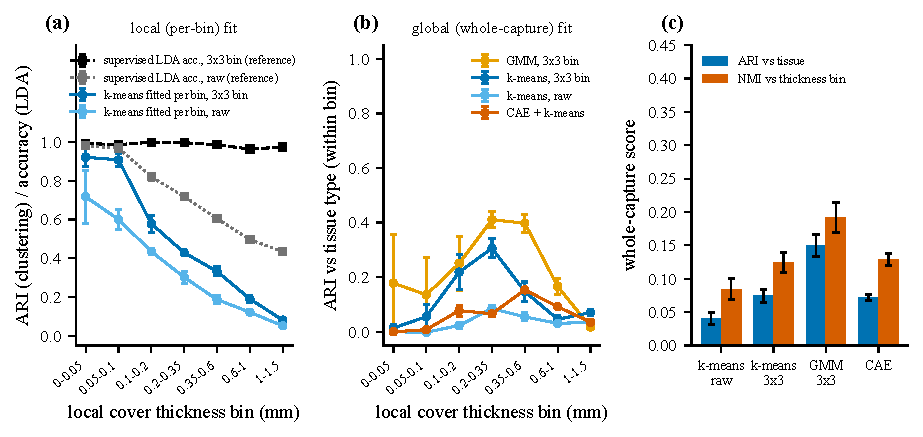
\includegraphics[width=0.8\textwidth]{E9_ari_vs_thickness.pdf}\\[2mm]
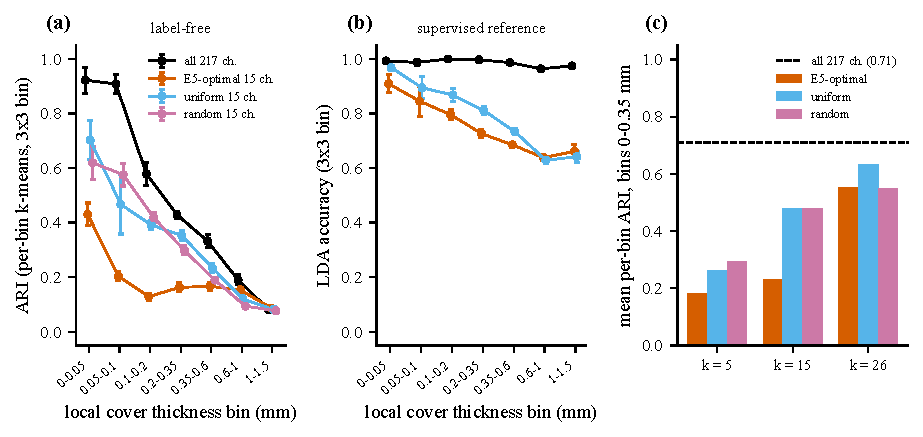
\includegraphics[width=0.8\textwidth]{E9_channels.pdf}
\caption{E9. \emph{Top:} clustering against burial, (a) per-bin ARI of $k$-means with and without binning and supervised LDA accuracy, (b) per-bin ARI of fits on the whole capture, (c) whole-capture ARI and NMI against tissue type and thickness bin. \emph{Bottom:} channel reduction, (a) label-free ARI and (b) supervised accuracy against thickness for 15 channels chosen by the E5 criterion, uniformly or at random, (c) mean ARI over 0--0.35~mm against $k$; the dashed line is the 217-channel value $0.71$.}
\label{fig:e9a}
\end{figure*}

\emph{Take-home.} Label-free separation of tissue types degrades monotonically with burial (ARI $0.92\to0.08$) although the information remains in the spectra, and channel sets designed for thickness are not suited to tissue classification.

\subsection{E10: Performance and convergence}
\todo{E10 results pending}

\section{Discussion and Limitations}
\label{sec:limits}
\textbf{What the tool is for.} The simulator is most useful where ground truth and controlled variation are needed: quantifying how a cover confounds a spectral ratio (E3), designing channel sets (E5), and benchmarking estimators and clustering methods (E7, E9). Whether its predictions transfer to real data depends on the fidelity of the twin, which Section~\ref{sec:v_s2r} documents, including that a non-parametric measured spectrum is as good a predictor as the calibrated model.

\textbf{Bounds are not precision.} The photon-limited CRLBs of E5 (sub-micron thickness) are bounds on information. Model bias dominates real retrieval: in E6 the RMSE is $160$--$260$~\textmu m at nominal exposure, $15$--$70\times$ the photon-limited tile bound, and the nominal $95\,\%$ intervals cover only $5$--$19\,\%$ of the tiles. The model-error term of Eq.~\eqref{eq:modelerr} brings the floor to $2$--$10$~\textmu m, still one to two orders below the observed errors, because it is a variance and not a bias. The relative error $\epsilon$ is an upper bound taken from sim-to-real residuals of collagen and droplets and is assumed independent across channels. The channel sets that are optimal depend on $\epsilon$ and on the estimand: sets chosen for thickness were worse than random for tissue classification (E9) and, on the phantom, for mapping (E6).

\textbf{Monte Carlo noise.} The 3D result is a Monte Carlo estimate (about $10\,\%$ rms per 0.5~mm face cell before smoothing; $2$--$3\,\%$ in a 3~mm region of interest), which is why studies report replicate noise floors. The `fast' mode used for datasets has a per-pixel tally noise of about $39\,\%$ per channel (median over channels), which affects the pixel-level analyses: it produced the artefactual floor of the first E7 version and part of the held-out E7 errors, and it contributes to the degradation of unbinned clustering in E9 (a separate check gives about $4\,\%$ Monte Carlo and $7\,\%$ sensor noise in a channel-mean-normalised metric, so the two figures are not comparable). Sobol' indices were estimated with $N=64$ base rows, so total indices are rank-level evidence only, and the group-index intervals are degenerate.

\textbf{Experimental design caveats.} E7 uses oracle endmember libraries built from the same pixels as the data; the held-out variant, which includes library-estimation noise, is the realistic one and is substantially worse beyond $0.4$~mm. Most experiments use a single scene family and a single noise realisation (E6, E7), one ROI (E5, E8) or one design of 14 captures (E9), and the surrogate used in E5 and E6 is trained on uniform blocks, so lateral transport at the wedge slope is unmodelled. The lateral blur of the wedge (E2) could not be resolved above the noise. The `autofluorescence fraction' of E2 uses the engine's own component bookkeeping and cannot be measured in real data without the cover alone. Voxel inclusions slow the 3D Monte Carlo by about $2\times$ (the $1.6\times$ target was not demonstrated on an idle machine), and they are index-matched to the host.

\textbf{Physics limitations.} Absorption and emission spectra of the dyes are parametric (Gaussians with skew and an optional vibronic shoulder), so there is no S$_0\!\to$S$_2$ band (fluorescein absorbs nothing at 405~nm in the model against about $3\,\%$ of its peak in reality), no exact mirror image and no solvent shift. Scattering is a power law with one Henyey--Greenstein $g$ per material, with no wavelength-dependent $g$, polarisation or coherence. Fluorescence has a single Stern--Volmer constant, FRET without overlap integral or orientation factor, one-generation isotropic secondary emission, only the 3400~cm$^{-1}$ water Raman band, and no lifetimes, depolarisation, temperature dependence or triplet saturation. Bleaching in the 1D engine uses the surface fluence. Block pixels have no secondary emission (fluorescence re-absorbed in the block is lost, making it a few percent to about $10\,\%$ dimmer for strongly overlapping dyes), a single camera direction per block, planar interfaces and a rectangular footprint. Tissue pigments measured in organic solvents are proxies for the bound pigments. The bottom of the block is a Fresnel interface to air and the stage never reflects. Indirect diffuse interreflection between objects is not implemented. Fisher information is a local bound that assumes an unbiased estimator and neglects fixed-pattern noise; calibration intervals are statistical, and the twin is calibrated on thin, dilute-equivalent samples, so collagen and droplet parameters are effective rather than intrinsic.

\textbf{Validation scope.} The validation is against analytic results, MCML-type benchmarks, an independent Monte Carlo and one laboratory's measurements; we have not compared 3D inclusion or tissue-phantom predictions with phantom measurements, and the cover-scene check of E8 uses thin measured samples. \todo{state any phantom measurement added before submission}

\section{Conclusion}
SpectralForge Studio couples a literature-grade layered-tissue 3D Monte Carlo with voxel inclusions, dye photophysics and a camera model with a study engine, inverse tools, information-theoretic design and calibration in one schema-driven, reproducible environment. The transport engine matches established benchmarks and an independent Monte Carlo to about one percent or better, and the calibrated twin predicts held-out excitation lines with a mean spectral angle of $8.4^\circ$, though not better than a copy of a measured spectrum. In simulations of collagen-covered tissue, the cover rather than metabolism dominates the optical redox ratio in this model (first-order share $0.66$ against $0.16$) and simple ratio corrections do not remove it; about 30 of 248 channels carry the information of the full protocol on cover thickness, but model bias, not photon noise, limits retrieval, so photon-limited bounds should be reported together with a model-error floor; and unmixing needs depth-matched endmembers between $0.1$ and $0.6$~mm and fails beyond, where the signal is below the noise. \todo{add inclusion-detectability (E4) and performance (E10) conclusions when complete}

\section*{Code Availability}
The source code, documentation, validation scripts and presets are available at \url{https://github.com/Nard248/spectral-select}.

\bibliographystyle{IEEEtran}
\bibliography{refs}
\end{document}
